\documentclass[draftspec]{sbmlpkgspec}

\newcommand{\ALL}{\noindent\fbox{\footnotesize \textbf{All}}\ }
\newcommand{\LRG}{\noindent\fbox{\footnotesize \textbf{LRG}}\ }
\newcommand{\SYM}{\noindent\fbox{\footnotesize \textbf{SYM}}\ }
\newcommand{\PN}{\noindent\fbox{\footnotesize \textbf{PN}}\ }
\newcommand{\sbml}[1]{\textsf{\textbf{#1}}} %def of sbml class names
\newcommand{\mathml}[1]{\texttt{\textbf{#1}}} %def of sbml class names
\newcommand{\attr}[1]{\textsf{#1}} %def of xml attributes
\newcommand{\const}[1]{\texttt{#1}} %def of xml constants
\newcommand{\type}[1]{\texttt{#1}} %def of xml/SBML types
\newcommand{\qualt}[1]{\textsf{\textbf{\hypertarget{#1}{#1}}}\textsf{\textbf{\hypertarget{#1s}{}}}} %def of sbml class names
\newcommand{\qual}[1]{\textsf{\textbf{\hyperlink{#1}{#1}}}} %call a L3F:qual class names
\newcommand{\listOf}[1]{\textsf{\textbf{\hyperlink{#1}{ListOf#1}}}} %call a L3F:qual class names

\newcommand{\Q}[1]{\indent\fbox{\textcolor{red}{Question: #1}} }
\newcommand{\A}[1]{\textcolor{lightblue}{Answer: #1} }
\newcommand{\TODO}[1]{\colorbox{lightblue}{\textcolor{white}{TODO: #1}}}

% setups and definitions of commands (end)

\begin{document}

\packageTitle{Qualitative Models}
\packageVersion{Version 1.0 (Draft)}
\packageVersionDate{29 Feb 2012}
\packageGeneralURL{http://sbml.org/Community/Wiki/SBML_Level_3_Proposals/Qualitative_Models}
\packageThisVersionURL{http://sbml.org/images/a/a7/SBML-L3-qual-specification_0.1.pdf}

\author{%
  \begin{tabular}{c>{\hspace{20pt}}c}
    Claudine Chaouiya			  & Martijn P. van Iersel\\[0.25em]
    \mailto{chaouiya@igc.gulbenkian.pt}	  & \mailto{mvpi@ebi.ac.uk}\\[0.25em]
    IGC Rua da Quinta Grande 6                & European Bioinformatics Institute\\
    P-2780-156 Oeiras                               & Cambridgeshire\\
    Portugal	                                            & UK\\
\\
\\
    Sarah M Keating\\[0.25em]\\
    \mailto{skeating@ebi.ac.uk}\\[0.25em]
    European Bioinformatics Institute\\
    Cambridgeshire\\
    UK\\
  \end{tabular}
}

\frontNotice{This is a working draft of the specification for the SBML Level 3
  package ``\texttt{qual}''.  It is not a normative document.  Please send
  comments and other feedback to the Package Working Group mailing list,
  \mailto{sbml-qual@lists.sourceforge.net}.}

\maketitlepage
\maketableofcontents

% -*- TeX-master: "sbml-level-2-version-4"; fill-column: 66 -*-
% $Id$
% $HeadURL$
% ----------------------------------------------------------------

\section{Introduction}
\label{sec:introduction}

We present the \textbf{S}ystems \textbf{B}iology \textbf{M}arkup
\textbf{L}anguage (SBML) Level~2 Version~\changed{\sbmlversion} Release~\changed{\sbmlrelease}, a model
representation format for systems biology.  SBML is oriented
towards describing systems of biochemical reactions of the sort
common in research on a number of topics, including cell signaling
pathways, metabolic pathways, biochemical reactions, gene
regulation, and many others.  SBML is defined in a neutral fashion
with respect to programming languages and software encoding;
however, it is primarily oriented towards allowing models to be
encoded using XML, the eXtensible Markup
Language~\citep{bosak:1999,bray:2000}.  This document contains
many examples of SBML models written in XML, as well as the text
of an XML Schema~\citep{biron:2000,fallside:2000,thompson:2000}
that defines SBML Level~2 Version~\changed{\sbmlversion}.  A
downloadable copy of the XML Schema and other related documents
and software are also available from the SBML project web site,
\url{http://sbml.org/}.

The SBML project is not an attempt to define a universal language
for representing quantitative models.  The rapidly evolving views
of biological function, coupled with the vigorous rates at which
new computational techniques and individual tools are being
developed today, are incompatible with a one-size-fits-all idea of
a universal language. A more realistic alternative is to
acknowledge the diversity of approaches and methods being explored
by different software tool developers, and seek a common
intermediate format---a \emph{lingua franca}---enabling
communication of the most essential aspects of the models.

The definition of the model description language presented here
does not specify \emph{how} programs should communicate or
read/write SBML.  We assume that for a simulation program to
communicate a model encoded in SBML, the program will have to
translate its internal data structures to and from SBML, use a
suitable transmission medium and protocol, etc., but these issues
are outside of the scope of this document.

%-----------------------------------------------------------------------------
\subsection{Developments, discussions, and notifications of updates}
%-----------------------------------------------------------------------------

% [MH 2006-03-06] This should still be changed to mention sbml-standard or
% whatever we use in the end, if we can decide in time for this spec.

SBML has been, and continues to be, developed in collaboration
with an international community of researchers and software
developers.  As in many projects, the primary mode of interaction
between members is electronic mail.  Discussions about SBML take
place on the mailing list
\link{http://sbml.org/forums}{sbml-discuss@caltech.edu}.  The
mailing list archives and a web browser-based interface to the
list are available at \url{http://sbml.org/forums/}.

A low-volume, broadcast-only mailing list is available 
where notifications of
revisions to the SBML speci\-fication, notices of votes on SBML
technical issues, and other critical matters are announced.  This
list is \link{http://sbml.org/forums}{sbml-announce@caltech.edu}
and anyone may subscribe to it freely.  This list will never be
used for advertising and its membership list will never be
disclosed.  \emph{It is vitally important that all users of SBML
  stay informed about new releases and other developments by
  subscribing to this list}, even if they do not wish to
participate in discussions on the
\link{http://sbml.org/forums}{sbml-discuss@caltech.edu} list.
Please visit the SBML project web site, \url{http://sbml.org/},
for information about how to subscribe to
\link{http://sbml.org/forums}{sbml-announce@caltech.edu} as well
as for access to the list archives.

In Section~\ref{sec:acknowledgements}, we attempt to acknowledge
as many contributors to SBML's development as we can, but as SBML
evolves, it becomes increasingly difficult to detail the
individual contributions on a project that has truly become an
international community effort.


%-----------------------------------------------------------------------------
\subsection{SBML Levels, Versions, and Releases}
\label{sec:levels-versions-releases}
%-----------------------------------------------------------------------------

Major editions of SBML are termed \emph{levels} and represent
substantial changes to the composition and structure of the
language.  The edition of SBML defined in this document, \sbmltwo,
represents an evolution of the language resulting from
the practical experiences of many users and developers working
with \sbmlone since since its introduction in the year
2001~\citep{hucka:2001,hucka:2003}.  All of the constructs of
Level~1 can be mapped to Level~2.  In addition, a subset of 
Level~2 constructs can be mapped to Level~1.  However, the
levels remain distinct; a valid SBML Level~1 document is not a
valid SBML Level~2 document, and likewise, a valid SBML Level~2
document is not a valid SBML Level~1 document.

Minor revisions of SBML are termed \emph{versions} and constitute
changes within a Level to correct, adjust, and refine
language features.  The present document defines SBML Level~2
Version~\changed{\sbmlversion}.  In Section~\ref{sec:notation-color}
  below explains how color is used in this document to
  indicate changes; a separate document provides a detailed
listing of the changes between versions of \sbmltwo as well as
between SBML Level~2 Version~\changed{\sbmlversion} and SBML Level~2 Version~\changed{3}.

Specification documents inevitably require minor editorial changes
as its users discover errors and ambiguities.  As a practical
reality, these discoveries occur over time.  In the context of
SBML, such problems are formally announced publicly as
\emph{errata} in a given specification document.  Borrowing
concepts from the World Wide Web Consortium~\citep{jacobs:2004},
we define SBML errata as changes of the following types: (a)
formatting changes that do not result in changes to textual
content; (b) corrections that do not affect conformance of
software implementing support for a given combination of SBML
Level and Version; and (c) corrections that \emph{may} affect such
software conformance, but add no new language features.  A change
that affects conformance is one that either turns conforming data,
processors, or other conforming software into non-conforming
software, or turns non-conforming software into conforming
software, or clears up an ambiguity or insufficiently documented
part of the specification in such a way that software whose
conformance was once unclear now becomes clearly conforming or
non-conforming~\citep{jacobs:2004}.  In short, errata do not
change the fundamental semantics or syntax of SBML; they clarify
and disambiguate the specification and correct errors.  (New
syntax and semantics are only introduced in SBML Versions and
Levels.)  An electronic tracking system for reporting and
monitoring such issues is available at
\url{http://sbml.org/issue-tracker}.

SBML errata result in new \emph{Releases} of the SBML
specification.  Each release is numbered with an integer, with the
first release of the specification being called release number~1.
Subsequent releases of an SBML specification document contain a
section listing the accumulated errata reported and corrected
since the first release.  A complete list of the errata for
\changed{\sbmltwofour} since the publication of Release~1 is also
made publicly available at
\url{http://sbml.org/specifications/sbml-level-2/version-\sbmlversion/errata/}.
Announcements of errata, releases of the SBML specification
and other major changes are made on the
\link{http://sbml.org/forums}{sbml-announce@caltech.edu} mailing
list.


%-----------------------------------------------------------------------------
\subsection{Language features and backward compatibility}
\label{sec:deprecated-features}
%-----------------------------------------------------------------------------

Some language features of previous SBML Levels and Versions have
been either deprecated or removed entirely in \changed{\sbmltwofour}.  For
the purposes of SBML specifications, the following are the
definitions of \emph{deprecated feature} and \emph{removed
  feature}:
\begin{description}
  
\item \emph{Removed language feature}: A syntactic construct that
  was present in previous SBML Levels and/or Versions within a
  Level, and has been removed beginning with a specific SBML Level
  and Version.  Models containing such constructs do not conform
  to the specification of that SBML Level and Version.
  
\item \emph{Deprecated language feature}: A syntactic construct
  that was present in previous SBML Levels and/or Versions within
  a Level, and while still present in the language definition, has
  been identified as non-essential and planned for future removal.
  Beginning with the Level and Version in which a given feature is
  deprecated, software tools should not generate SBML models
  containing the deprecated feature; however, for backward
  compatibility, software tools reading SBML should support the
  feature until it is actually removed.

\end{description}

As a matter of SBML design philosophy, the preferred approach to
removing features is by deprecating them if possible.  Immediate
removal of SBML features is not done unless serious problems have
been discovered involving those features, and keeping them would
create logical inconsistencies or extremely difficult-to-resolve
problems.  The deprecation or outright removal of features in a
language, whether SBML or other, can have significant impact on
backwards compatibility.  Such changes are also inevitable over
the course of a language's evolution.  SBML must by necessity
continue evolving through the experiences of its users and
implementors.  Eventually, some features will be deemed unhelpful
despite the best intentions of the language editors to design a
timeless language.

Throughout the SBML specification, removed and deprecated features
are discussed in the text of the sections where the features
previously appeared.  Appendix~\ref{apdx:changes}
lists the changes and describes their motivations in more detail.


%-----------------------------------------------------------------------------
\subsection{Document conventions}
\label{sec:notation}
%-----------------------------------------------------------------------------

In this section, we describe the conventions we use in this
specification document in an effort to communicate information
more effectively and consistently.


\subsubsection{Color conventions}
\label{sec:notation-color}

Throughout this document, we use coloring to carry additional
information for the benefit of those viewing the document on media
that can display color:

\begin{itemize}

\item We use red color in text and figures to indicate changes
  between this version of the specification (\sbmltwo Version~\changed{\sbmlversion} Release~\changed{\sbmlrelease}) and the
  \emph{most recent previous version} of the specification (which,
  for the present case, is \changed{\sbmltwothree Release~2}).  The changes
  may be either additions or deletions of text; in the case of
  deletions, entire sentences, paragraphs or sections are colored
  to indicate a change has occurred inside them.

\item We use blue color in text to indicate a hyperlink from one
  point in this document to another.  Clicking your computer's
  pointing device on blue-colored text will cause a jump to the
  section, figure, table or page to which the link refers.  (Of
  course, this capability is only available when using electronic
  formats that support hyperlinking, such as PDF and
  HTML.)

\end{itemize}


\subsubsection{Typographical conventions for names}
\label{sec:notation-typographical}

The following typographical notations are used in this document to
distinguish objects and data types from other kinds of entities:

\begin{description}
  
\item \abstractclass{AbstractClass}: Abstract classes are classes
  that are never instantiated directly, but rather serve as
  parents of other classes.  Their names begin with a capital
  letter and they are printed in a slanted, bold,
  sans-serif typeface.  In electronic document formats, the class
  names are also hyperlinked to their definitions in the
  specification.  For example, in the PDF and HTML versions of
  this document, clicking on the word \SBase will send the reader
  to the section containing the definition of this class.
  
\item \class{Class}: Names of ordinary (concrete) classes begin
  with a capital letter and are printed in an upright,
  bold, sans-serif typeface.  In electronic document
  formats, the class names are also hyperlinked to their
  definitions in the specification.  For example, in the PDF and
  HTML versions of this document, clicking on the word \Species
  will send the reader to the section containing the definition of
  this class.

\item \token{SomeThing}, \token{otherThing}: Attributes
  of classes, data type names, literal XML, and generally all
  tokens \emph{other} than SBML UML class names, are printed in an
  upright typewriter typeface.  Primitive types defined by SBML
  begin with a capital letter, but unfortunately, \xmlschemaone
  does not follow any convention and primitive XML types may
  either start with a capital letter (e.g,.  \primtype{ID}) or not
  (e.g., \primtype{double}).

\end{description}


\subsubsection{UML notation}
\label{sec:notation-uml}

% fixme: use primary citations for UML below

Previous specifications of SBML used a notation that was at one
time (in the days of \sbmlone) fairly close to UML, the Unified
Modeling Language~\citep{eriksson:1998,oestereich:1999}, though
many details were omitted from the UML diagrams themselves.  Over
the years, the notation used in successive specifications of SBML
grew increasingly less UML-like.  Beginning with \sbmltwothree, we
have completely overhauled the specification's use of UML and once
again define the XML syntax of SBML using, as much as possible, proper
and complete UML~1.0.  We then systematically map this UML
notation to XML, using \xmlschemaone~\citep{biron:2000,fallside:2000,thompson:2000} to express
the overall syntax of SBML.  In the rest of this section, we
summarize the UML notation used in this document and explain the
few embellishments needed to support transformation to XML form.
A complete Schema for SBML is given in Appendix~\ref{apdx:schema}.

We see three main advantages to using UML as a basis for defining
SBML data objects.  First, compared to using other notations or
a programming language, the UML visual representations are
generally easier to grasp by readers who are not computer
scientists.  Second, the notation is implementation-neutral: the
objects can be encoded in any concrete implementation
language---not just XML, but C, Java and other languages as well.
Third, UML is a de facto industry standard that is documented in
many resources.  Readers are therefore more likely to be familiar
with it than other notations.


\paragraph{Object class definitions}

Object classes in UML diagrams are drawn as simple tripartite
boxes, as shown in Figure~\ref{fig:simple-class-eg} (left).  UML
allows for operations as well as data attributes to be defined,
but SBML only uses data attributes, so all SBML class diagrams use
only the top two portions of a UML class box (see the right-hand
diagram of Figure~\ref{fig:simple-class-eg}).

\begin{figure}[htb]
  \centering
  \small
  \begin{classbox}{Class Name}
    attributes\\
    \hline
    operators\\
  \end{classbox}
  \quad  \quad  \quad  \quad
  \begin{classbox}{ExampleClass}
    attribute: int \\
    anotherAttribute: double\\
  \end{classbox}
  \caption{(Left) The general form of a UML class
      diagram.  (Right) Example of a class diagram of the sort
      seen in SBML.  SBML classes never use operators, so SBML
      class diagrams only show the top two parts.}
  \label{fig:simple-class-eg}
\end{figure}

As mentioned above, the names of ordinary (concrete) classes begin
with a capital letter and are printed in an upright,
bold, sans-serif typeface.  The names of attributes
begin with a lower-case letter and generally use a mixed case
(sometimes called ``camel case'') style when the name consists of
multiple words.  Attributes and their data types appear in the
part below the class name, with one attribute defined per line.
The colon character on each line separates the name of the
attribute (on the left) from the type of data that it stores (on
the right).  The subset of data types permitted for SBML
attributes is given in Section~\ref{sec:primitive-types}.

In the right-hand diagram of Figure~\ref{fig:simple-class-eg}, the
symbols \token{attribute} and \token{anotherAttribute} represent
attributes of the object class \class{ExampleClass}.  The data
type of \token{attribute} is \primtype{int}, and the data type of
\token{anotherAttribute} is \primtype{double}.  In the scheme used
by SBML for translating UML to XML, object attributes map directly
to XML attributes.  Thus, in XML, \class{ExampleClass} would yield
an element of the form \token{<\emph{element} attribute="42"
  anotherAttribute="10.0">}.

Notice that the element name is not \token{<ExampleClass ...>}.
Somewhat paradoxically, the name of the element is \emph{not} the
name of the UML class defining its structure.  The reason for this
may be subtle at first, but quickly becomes obvious: object
classes define the form of an object's \emph{content}, but a class
definition by itself does not define the \emph{label} or symbol
referring to an instance of that content.  It is this label that
becomes the name of the XML element.  In XML, this symbol is most
naturally equated with an element name.  This point will hopefully
become more clear with additional examples below.


\paragraph{Subelements}

We use UML composite aggregation to indicate a class object can
have other class objects as parts.  Such containment hierarchies
map directly to element-subelement relationships in XML.
Figure~\ref{fig:subelement-eg} gives an example.

\begin{figure}[htb]
  \centering
  \small
  \begin{tikzpicture}[level distance=0.7in]
    \node[left=0.3in] (a) {
      \begin{classbox}{Whole}
        A: int \\
        B: string \\
      \end{classbox}
    };
    \node[right=0.3in] (b) {
      \begin{classbox}{Part}
        C: double \\
      \end{classbox}
    };
    \draw[diamond-,shorten >=-6pt] (a) -- (b)
      node[left=0.8in,above=2pt] {\textsf{inside}};
  \end{tikzpicture}
  \caption{Example illustrating composite
      aggregation: the definition of one class of objects
      employing another class of objects in a part-whole
      relationship.  In this particular example, an instance of a
      \class{Whole} class object must contain exactly one instance
      of a \class{Part} class object, and the symbol referring to
      the \class{Part} class object is \token{inside}.  In XML,
      this symbol becomes the name of a subelement and the content
      of the subelement follows the definition of \class{Part}.}
  \label{fig:subelement-eg}
\end{figure}

The line with the black diamond indicates composite aggregation,
with the diamond located on the ``container'' side and the other
end located at the object class being contained.  The label on the
line is the symbol used to refer to instances of the contained
object, which in XML, maps directly to the name of an XML element.
The class pointed to by the aggregation relationship (\class{Part}
in Figure~\ref{fig:subelement-eg}) defines the \emph{contents} of
that element.  Thus, if we are told that some element named
\token{barney} is of class \token{Whole}, the following is an
example XML fragment consistent with the class definition of
Figure~\ref{fig:subelement-eg}:

\begin{example}
<barney A="110" B="some string">
    <inside C="444.4">
</barney>
\end{example}

Sometimes numbers are placed above the line near the ``contained''
side of an aggregation to indicate how many instances can be
contained.  The common cases in SBML are the following:
\token{[0..*]} to signify a list containing zero or more;
\token{[1..*]} to signify a list containing at least one; and
\token{[0..1]} to signify exactly zero or one.  The absence of a
numerical label means ``exactly 1''.  This notation appears
throughout this specification document.


\paragraph{Inheritance}

\begin{wrapfigure}[18]{r}{1.9in}
  \centering
  \small
  \vspace*{-7ex}
  \begin{tikzpicture}[level distance=0.75in]
    \node { 
      \begin{classbox}{Parent}
        A: int           \\
        B: boolean \\
      \end{classbox}
    }
    [open triangle 60-,edge from parent fork down,sibling distance=2.15in]
    child {node (a) {
        \begin{classbox}{Child}
          C: int \\
          D: string \\
        \end{classbox}
      }}
    ;
  \end{tikzpicture}
  \caption{Inheritance.}
  \label{fig:inheritance-eg}
\end{wrapfigure}
Classes can inherit properties from other classes.  Since SBML
only uses data attributes and not operations, inheritance in SBML
simply involves data attributes from a parent class being
inherited by child classes.  Inheritance is indicated by a line
between two classes, with an open triangle next to the parent
class; Figure~\ref{fig:inheritance-eg} illustrates this.  In this
example, the instances of object class \class{Child} would have
not only attributes \token{C} and \token{D}, but also attributes
\token{A} and \token{B}.  All of these attributes would be
required (not optional) on instances of class \class{Child}
because they are mandatory on both \class{Parent} and
\class{Child}.



\paragraph{Additional notations for XML purposes}

Not everything is easily expressed in plain UML.  For example, it
is often necessary to indicate some constraints placed on the
values of an attribute.  In computer programming uses of UML, such
constraints are often expressed using Object Constraint Language
(OCL), but since we are most interested in the XML rendition of
SBML, in this specification we use \xmlschemaone (when possible)
as the language for expressing value constraints.  Constraints on
the values of attributes are written as expressions surrounded by
braces (\{ \}) after the data type declaration, as in the example
of Figure~\ref{fig:unit-eg}.

\begin{figure}[htb]
  \centering
  \small
  \vspace*{-1ex}
  \begin{tikzpicture}[level distance=0.7in]
    \node { \emptyClassbox{\textsl{SBase}} }
      [open triangle 60-,edge from parent fork down,sibling distance=2.5in]
      child {node (a) {
          \begin{classbox}{Sbml}
            level: positiveInteger \{ use="required" fixed="2" \}   \\
            version: positiveInteger \{ use="required" fixed="\changed{4}" \} \\
          \end{classbox}
        }}
      child {node (b) {
          \emptyClassbox{Model}
        }}
     ;
     \draw[diamond-] (a) -- (b) 
       node[above=6pt,left=40pt] {\textsf{model}};
  \end{tikzpicture}
  \caption{A more complex example definition drawing on
      the concepts introduced so far in this section.  Both
      \class{Sbml} and \class{Model} are derived from
      \abstractclass{SBase}; further, \class{Sbml} contains a
      single \class{Model} object named \token{model}.  Note the
      constraints on the values of the attributes in \class{Sbml};
      they are enclosed in braces and written in XML Schema
      language.  The particular constraints here state that both
      the \token{level} and \token{version} attributes must be
      present, and that the values are fixed as indicated.}
  \label{fig:unit-eg}
\end{figure}

In other situations, when something cannot be concisely expressed
using a few words of XML Schema, we write constraints using
English language descriptions surrounded by braces (\{ \}).  To
help distinguish these from literal XML Schema, we set the English
text in a slanted typeface.  The text accompanying all SBML
component definitions provides explanations of the constraints and
any other conditions applicable to the use of the components.


\paragraph{Compatibility issues and warnings}

One important and confusing point that goes against the grain of
XML must be highlighted: the order in which subelements appear
within SBML elements \emph{is} significant and \emph{must} follow
the order given in the corresponding object definition.  This
ordering is also difficult to express in plain UML, so we resort
to using the approach of stating ordering requirements as
constraints written in English and (again) enclosed in
braces (\{ \}).  Figure~\vref{fig:sbase} gives an example of this.

The ordering restriction also holds true when a subclass inherits
attributes and elements from a base class: the base class
attributes and elements must occur before those introduced by the
subclass.

This ordering constraint stems from aspects of XML Schema beyond
our control (specifically, the need to use XML Schema's
\token{sequence} construct to define the object classes).  It is
an occasional source of software compatibility problems, because
validating XML parsers will generate errors if the ordering
within an XML element does not correspond to the SBML object class
definition.

\section{Background and context}
\label{background}
Currently, there is no official way of encoding the layout of 
computational models in SBML. Software tools wishing to share this 
information have been using the SBML annotation scheme to store this 
information in proprietary form. 

The layout proposal was made in early 2003, since then it has been 
incorporated into libSBML (\cite{Gauges01082006}) and has been used by 
software applications (e.g.: \cite{COPASI}, \cite{sbw}) for SBML Level~2 
and Level~3. 

The overall structure of this proposal reflects design decisions that 
will be detailed in this section. These decisions are mainly based on 
the discussion on the mailing list and during the workshop in St. Louis. 
It was requested that several layouts should be stored in one SBML file. 
And so the layout is stored in a \ListOfLayouts as child of the the 
\Model element instead of direct annotations to the model constituents. 


\begin{center}
\begin{figure}[!h]
\begin{center}
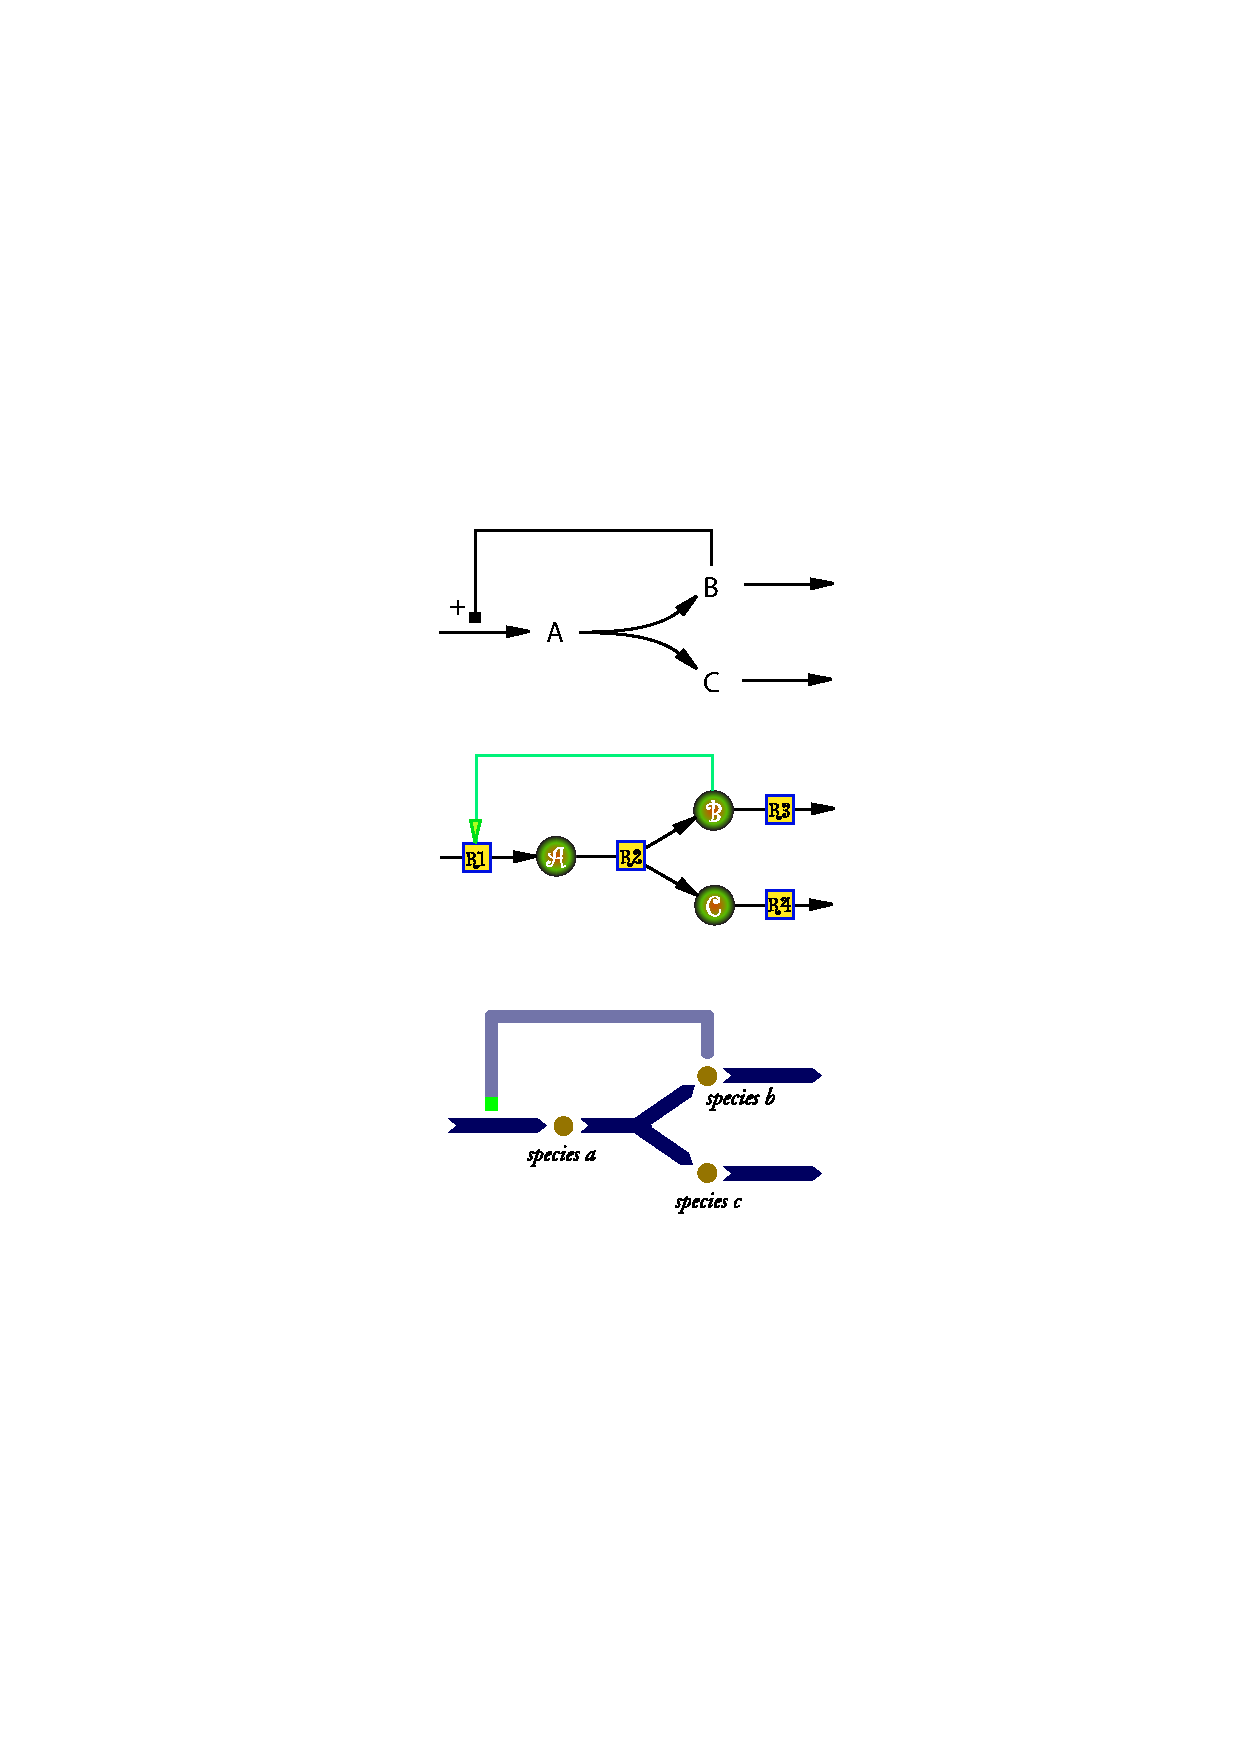
\includegraphics[scale=1]{figures/layout1}
\end{center}
\caption{Illustration of different renderings of the same layout.}
\label{UML:All}
\label{figure:rendering}
\end{figure}
\end{center}

The layout of a reaction network diagram should be described as 
graphical representations of species and reactions (and not as arbitrary 
drawing or graph). This means that existing languages for the 
description of vector drawings (SVG) or general graphs cannot be used. 
While it may seem unnecessary to invent a new language when an existing 
one like SVG could in principle be used to describe the layout of a 
reaction network, there are good reasons to have a language tailored 
specifically for the layout of SBML models. 

Presumably, most programs that will use this SBML extension are 
primarily programs dealing with biochemical models. Internally, they 
will have data structures for species and reactions, so it will be 
natural for them to describe the layout of the reaction network also in 
terms of species and reactions (and not in terms of polygons or 
splines). Thus the \token{layout} object has a similar structure like 
the SBML \token{model} object and contains lists of graphical 
representations of compartments, species, and reactions (called 
\token{compartmentGlyph, speciesGlyph,} and \token{reactionGlyph} 
respectively). Additional layout elements and relationships can be 
represented by using the \token{graphicalObject} and 
\token{generalGlyph} elements. 

Another important question is the level of detail that the description 
should provide. For simplicity, only the layout (i.e., the position of 
the different graphical objects) of the diagram is encoded, not the 
details of how it should be rendered. That is left to the SBML Level~3 
Render package. 

\ref{figure:rendering} illustrates this distinction. All three diagrams 
could be renderings of the same layout and would be described by 
identical SBML files. No information about colors, line styles, fonts, 
etc., is present in the layout description. 

The next question is how the relation between the model and the layout 
should be established. There seems to be consensus that one model 
element can be represented by several layout elements. For example, it 
can be useful to have several representations of one species in the 
layout to avoid crossing lines. This can be accomplished if every layout 
element has a field that refers to the id of a model element. 

There are also cases where a layout element does not correspondent to 
exactly one model element. One example would be if a layout shows a 
simplified version of the model where one reaction in the layout 
corresponds to several reactions and intermediate species in the model. 
This is the reason why the field in the layout elements that refers to 
the model elements is optional, allowing layout objects that do not have 
a specific counterpart in the SBML model. 

The result of all this is a way to describe a graphical layout of a 
reaction network in biochemical terms. This layout can be closely tied 
to the biochemical model. A graphical model editor for example would 
typically create a layout that is closely connected (by a one-to-several 
relation from the model elements to the layout elements) to the model. 

A more general layout design program could also create a layout that is 
not so closely tied to the model, for example, it could create a layout 
that shows a simplified version of the model. 


% -*- TeX-master: "main"; fill-column: 72 -*-

\newcommand{\fixttspace}{\hspace*{1pt}}

\section{Package syntax and semantics}

In this section, we define the syntax and semantics of the Qualitative Models package for SBML Level~3 Version~1.  We expound on the
various data types and constructs defined in this package, then in
\sect{examples}, we provide complete examples of using the constructs in
example SBML models.

\subsection{Namespace URI and other declarations necessary for using this package}
\label{xml-namespace}

Every SBML Level~3 package is identified uniquely by an XML namespace
URI.  For an SBML document to be able to use a given SBML Level~3
package, it must declare the use of that package by referencing its URI.
The following is the namespace URI for this version of the Qualitative Models package for SBML Level~3 Version~1:
\begin{center}
\uri{http://www.sbml.org/sbml/level3/version1/qual/version1}
\end{center}

In addition, SBML documents using a given package must indicate whether
understanding the package is required for complete mathematical
interpretation of a model, or whether the package is optional.  This is
done using the attribute \token{required} on the \token{<sbml>} element
in the SBML document.  For the Qualitative Models package,
the value of this attribute must be set to \val{true}.

The following fragment illustrates the beginning of a typical SBML model
using SBML Level~3 Version~1 and this version of the Qualitative Models package:

\begin{example}
<?xml version="1.0" encoding="UTF-8"?>
<sbml xmlns="http://www.sbml.org/sbml/level3/version1/core" level="3" version="1"
      xmlns:qual="http://www.sbml.org/sbml/level3/version1/qual/version1" qual:required="true">
\end{example}
    

% -----------------------------------------------------------------------------
\subsection{Primitive data types}
\label{primitive-types}

Section~3.1 of the SBML Level~3 specification defines a number of
primitive data types and also uses a number of XML Schema 1.0 data
types \citep{biron:2000}.  We assume and use some of them in the rest of
this specification, specifically \primtype{boolean}, \primtype{ID},
\primtype{SId}, \primtype{SIdRef}, and \primtype{string}. The Qualitative Model package defines other primitive types;
they are described below.

% removed for now
%\subsubsection{Type \fixttspace\primtypeNC{temporisationType}}
%\label{primtype-temporisation}
%
%The \primtype{temporisationType} is an enumeration of values used to indicate the updating policy used by %a \Transition.  The possible values are \const{timer}, \const{priority}, \const{sustain}, \const{proportion} %and \const{rate}.
%
\subsubsection{Type \fixttspace\primtypeNC{sign}}
\label{primtype-sign}

The \primtype{sign} is an enumeration of values used to indicate direction of an \Input within the system.  The possible values are \const{positive}, \const{negative}, \const{dual} and \const{unknown}. 

\subsubsection{Type \fixttspace\primtypeNC{transitionInputEffect}}
\label{primtype-inputeffect}
The \primtype{transitionInputEffect} is an enumeration of values used to indicate the effect of an \Input \Transition within the system.  The possible values are \const{none} and \const{consumption}.

\subsubsection{Type \fixttspace\primtypeNC{transitionOutputEffect}}
\label{primtype-outputeffect}
The \primtype{transitionOutputEffect} is an enumeration of values used to indicate the effect of an \Output \Transition within the system.  The possible values are \const{production} and \const{assignmentLevel}.

\pagebreak
% -----------------------------------------------------------------------------
\subsection{Qualitative modelling}
\label{qual}

Before describing the classes and their attributes that have been used by this Qualitative Models Specification it is worth clarifying the intended meaning of some of the terms used. 

\subsubsection{Levels}

%\TODO{need to address the issue of still allowing symbols in a simple form}

The entities being modelled have a \emph{level} associated with them that indicates the current state of the entity. A \emph{level} is an integer and takes values that range from \val{0} up to and including a maximum.

In future versions of the Qualitative Modelling specification, it is intended to introduce a means of specifying symbols to represent any value that might be appropriate in the model (see ~\sec{apdx:apdx-future}).

%A \emph{symbol} is intended to represent any value that might be appropriate in the model.  A user can %merely define the set of symbols that might be used and how the \token{symbolValue} associated with an %entity might be altered  by the model. 
\smallskip

\subsubsection{Transitions}

Qualitative Models consider \emph{transitions} that alter the levels of entities involved in the model, depending on the level of some other entities.  This may involve the level of an entity being increased or decreased by a fixed amount; the level remaining unchanged; or the level being reassigned to an alternate value. Transitions occur when a set of conditions is met. These conditions may involve the levels falling above or below  a given \emph{threshold}. 

A simple example of this is the case where there are two entities A and B and the model states that when the level of A exceeds \val{1} (the threshold), the level of B is increased by \val{1}. 

\subsubsection{FunctionTerms}

The resulting value of an entity affected by a transition may have several possibilities that are governed by a number of conditions. Each transition can have a list of conditional functions \emph{functionTerms}, each associated with a result that allow the user to specify sets of piecewise conditions. For example a model may wish to encode the following
\smallskip
\begin{center}
$B = \left\{ \begin{array}{ll}
      B+1 & \mbox{if $A < 1$} \\
      B & \mbox{if $1 <= A < 3$} \\
     B + 2 & \mbox{otherwise}  \\
     \end{array}
\right.
$
\end{center}

\smallskip
In this case the \Transition would have a \FunctionTerm for each of the first two conditions and a \DefaultTerm for the otherwise component.


\subsubsection{Interpretation of time}


Transitions occur when a set of conditions are met.  This specification assumes that these conditions are not dependent on time and can occur at any arbitary time point.  Thus the use of any math that explicitly involves time (e.g. the \token{csymbol} \textbf{time} or \textbf{delay}) is not recommended. It is anticipated that future versions will consider time issues see \sec{apdx:apdx-future}.



\subsubsection{Hybrid models}


It is noted in \sec{apdx:apdx-future} that this specification does not facilitate the use of SBML constructs outside the scope of this package within a particular model.  This is an aspect of modelling that will be addresses in future versions.







% -----------------------------------------------------------------------------
\subsection{The extended \class{Model} class}
\label{model-class}

The extension of SBML Level~3 Core's \Model class is relatively
straightforward: the Qualitative Models Package adds two lists,
one for holding qualitativeSpecies (\token{listOfQualitativeSpecies}, of class
\ListOfQualitativeSpecies), and the other for holding transitions (\token{listOfTransitions},
of class \ListOfTransitions).  \fig{qual-extended-model-uml} provides the UML
diagram.  

\pagebreak

The \sbml{Model} element may contain at most one \ListOfQualitativeSpecies, which must contain at least one \QualitativeSpecies. It may also contain at most one \ListOfTransitions which must contain at least one \Transition.The \QualitativeSpecies class and
the \Transition  class are defined in \sect{qualSpecies-class} and \sect{transitions-class} respectively.

\begin{figure}[h!]
  \includegraphics{figs/qual-extended-model-uml.pdf}
  \caption{The definitions of the extended \Model class. In other respects, \Model remains defined as
    in the SBML Level~3 Core specification.}
  \label{qual-extended-model-uml}
\end{figure}


% -----------------------------------------------------------------------------
\subsection{The \class{QualitativeSpecies} class}
\label{qualSpecies-class}
Similarly to the \sbml{Species} in SBML, the components of qualitative models refer to pools of entities that are considered indistinguishable and are each located in a specific \sbml{Compartment}. However, here components are characterised by their qualitative influences rather than by taking part in reactions. Therefore, we define the \QualitativeSpecies element to represent such pools of entities.

In a Petri net, {\em qualitative species} refer to the places of the model, while in a logical model, they refer to the variables of this model (i.e. nodes of the influence graph).

A \QualitativeSpecies describes a pool of indistinguishable entities in a \sbml{Compartment}. It is associated with  a \token{level} (an integer representing e.g. an activity state, or a functional level of concentration, etc.)  %or a \token{symbolValue} from its \ListOfSymbolicValues.
 The \QualitativeSpecies class is defined in \fig{qual-qualitative-species-uml}.
%\TODO{add listOfSymbols back}
\begin{figure}[h]
  \includegraphics{figs/qual-qualitative-species-uml.pdf}
  \caption{The definitions of the \QualitativeSpecies class. }
  \label{qual-qualitative-species-uml}
\end{figure}

\paragraph{The \fixttspace\token{id} attribute}

The \token{id} attribute takes a required value
of type \primtype{SId}. The \token{id} is used as an identifier for the particular \QualitativeSpecies. It can be used as a 
<ci> element within math elements included by elements defined within the namespace of the Qualitative Models specification i.e. the \token{math} element of a \FunctionTerm, in which case it it interpreted as the \emph{level} of this \QualitativeSpecies. Note that for SBML Level~3 Version~1 identifiers from a given package cannot be referenced by elements outside that package. 

\paragraph{The \fixttspace\token{name} attribute}

A \QualitativeSpecies also has an optional \token{name} attribute of type \primtype{string}. 
 The \token{name} attribute should be used
in the same manner as on SBML Level~3 Core
objects; see Section~3.3.2 of the SBML Level~3 Version~1 Core
specification for more information.


\paragraph{The \token{compartment} attribute}
The required attribute \token{compartment}, of type \primtype{SIdRef}, is used to identify the compartment in which the qualitativeSpecies is located.  The attribute's value must be the identifier of an existing \sbml{Compartment} object in the model.  This attribute is comparable with the \token{compartment} attribute on the \sbml{Species} element.

\paragraph{The \token{constant} attribute}
The required attribute \token{constant}, of type \primtype{boolean}, is used to indicate that the \token{level} of the qualitativeSpecies is fixed or can be varied. This attribute is comparable with the \token{constant} attribute on the \sbml{Species} element.

Typically, in a regulatory or influence graph a \QualitativeSpecies may receive no interaction and if so, would appear only as an \Input in the model and have the value of the \token{constant} attribute set to \val{true}. In other influence graphs or in Petri net models a \QualitativeSpecies may occur as an \Input whose level is changed by the \Transition and would have \token{constant} set to \val{false}.  The nature of changes to a \QualitativeSpecies resulting from a \Transition is also recorded using the \token{transitionEffect} attribute on the \Input (see section \ref{input-class}) and may be set to \val{none} to indicate there is no change. This duplication of information provides a means of validating the modeller's intent and also allows entities on the borders of a system to be easily identified.
 


\paragraph{The \token{initialLevel}  attribute}
The \token{initialLevel} is a non-negative \primtype{integer} that defines the initial \emph{level} of the \QualitativeSpecies in its \sbml{Compartment}. This attribute is optional but cannot exceed the value of the \token{maxlevel} attribute, if both are set.

\paragraph{The \token{maxLevel} attribute}
The \token{maxLevel} is a non-negative \primtype{integer} that sets the maximal \emph{level} of the \qualt{QualitativeSpecies}. This attribute is optional but when set, the \emph{level} of the \QualitativeSpecies must not exceed this value at any point in a simulation.

In logical models, the \token{maxLevel} should be coherent with the \token{resultLevel} values in the function terms defined for the corresponding transition, i.e. the model must not contain a \FunctionTerm that attempts to set a \emph{level} that exceeds this value.

In Petri nets, this attribute is meant to define place capacities. Hence, a transition is not enabled if the value resulting from its firing would exceed the  \token{maxLevel} of one of its output places.  The attribute is not required and even if explicitly stated, the restriction imposed by place capacities in a Petri net model  \textbf{must} be encapsulated within the \token{math} element of the \FunctionTerm elements. 

This attribute can also be used to indicate the range of possible levels for a \QualitativeSpecies whose \token{constant} attribute is true. This may seem a little contradictory, since if the \token{constant} attribute is true then the level associated with the \QualitativeSpecies cannot vary. However, it provides additional information regarding the possible levels particularly in the case where no \token{initialLevel} has been set.

%\subsubsection{The \class{SymbolicValue} class}
%The \QualitativeSpecies element may contain at most one \ListOfSymbolicValues that contains zero or more %\SymbolicValue elements. An empty list is allowed, and useful for e.g. adding annotations.
%
%The \SymbolicValue element defines a non instantiated parameter that allows the model to associate %undefined values with a particular \QualitativeSpecies.
%Symbols can be considered as uninstantiated parameters. Such symbols may represent the different %solutions of piecewise linear differential equations, along with different thresholds.
%
%\paragraph{The \token{id} attribute}
%A \SymbolicValue element has an \token{id} attribute that takes a required value
%of type \primtype{SId}. The \token{id} is used as an identifier for the particluar \SymbolicValue and may be %referenced by the \token{symbolicResult} attribute of a \FunctionTerm within a \Transition to indicate that %this \SymbolicValue is the resulting value for this \QualitativeSpecies following a particular \Transition.
%
%\paragraph{The \token{name} attribute}
%There is an optional \token{name} attribute of type \primtype{string} that should be used
%in the same manner as on SBML Level~3 Core
%objects; see Section~3.3.2 of the SBML Level~3 Version~1 Core
%specification for more information.
%
%
%\paragraph{The \token{rank} attribute}
%The \token{rank} is an \primtype{integer} that defines the position of the symbol in the \ListOfSymbolicValues. This attribute is optional. \Q{What difference does the position make or does rank meaning ordering independent of physical position ?}
%
%\Q{Are symbols and levels exclusive?}

\pagebreak


% -----------------------------------------------------------------------------
\subsection{The \class{Transition} class}
\label{transitions-class}
A \Transition element contains at most one \ListOfInputs and one \ListOfOutputs and exactly one \ListOfFunctionTerms. These objects classes are defined in \fig{qual-transition-uml}.

\begin{figure}
  \includegraphics{figs/qual-transition-uml.pdf}
  \caption{The definitions of \Transition, \Input, \Output, \DefaultTerm and \FunctionTerm classes. Note that the \DefaultTerm class is not derived from SBase. }
  \label{qual-transition-uml}
\end{figure}


A \Transition defines the changes in \emph{level} associated with the \QualitativeSpecies  that occur when a \Transition is enabled.  


\pagebreak


In logical models a \Transition is used to specify the logical rule associated with a \QualitativeSpecies (that appears as an \Output of this \Transition). For example, the rule $if A > 1: B = 2$ would be encapsulated as a \Transition with \QualitativeSpecies \val{A} as an \Input and \val{B} as an \Output.


In Petri net models a \Transition is interpreted, using the common Petri net semantics, as events that might occur within the system causing tokens to be moved. The example  in \sec{sub:ex_pn} illustrates a simple Petri net model with two input places, two output places and one transition.



\paragraph{The \token{id} attribute}
A \Transition element has an optional \token{id} attribute of type \primtype{SId}.  In constrast to most SBML classes the \token{id} attribute on a \Transition has no mathematical interpretation.

\paragraph{The \token{name} attribute}
There is an optional \token{name} attribute of type \primtype{string} that should be used
in the same manner as on SBML Level~3 Core
objects; see Section~3.3.2 of the SBML Level~3 Version~1 Core
specification for more information.

%\paragraph{The \token{temporisationType} attribute}
%A \Transition has an attribute \token{temporisationType} of type \primtype{temporisationType} used to indicate the updating policy associated with this \Transition element. This attribute is optional. \tab{transition-temporisation} describes the different updating policies.
%
%\begin{table}[thb]
%  \begin{edtable}{tabular}{p{1in}p{5in}}
%    \toprule
%    \textbf{TemporisationType} & \textbf{Interpretation} \\
%    \midrule
%    \const{timer} & TBD \\
%    \const{priority} & TBD \\
%    \const{sustain} & TBD \\
%    \const{proportion} & TBD \\
%    \const{rate} & TBD \\
%    \bottomrule
%  \end{edtable}
%  \caption{Interpretation of the \token{temporisationType} attribute on a \Transition.} 
%  \label{transition-temporisation}
%\end{table}
%
%\TODO{need more explanation of this}

\subsubsection{The \class{Input} class}
\label{input-class}
The \ListOfInputs contains at least one element of type \Input. 
%A transition with zero inputs can be useful for defining an initial assignment, where the state of an output %depends on a function but not on any input values. An empty list is allowed, and useful for e.g. adding %annotations.
Each \Input refers to a \QualitativeSpecies that participates in the corresponding \Transition.
In Petri nets, these are the input places of the transition. In logical models, they are the regulators of the species whose behaviour is defined by the transition.

\paragraph{The \token{id} attribute}
An \Input element has an optional \token{id} attribute of type \primtype{SId}. The identifier of an \Input can be used as a 
<ci> element within 
math elements included by elements defined within the namespace of the Qualitative Models specification i.e. the \token{math} element of a \FunctionTerm, in which case it it interpreted as the \token{thresholdLevel} of this \Input. Note that for SBML Level~3 Version~1 identifiers from a given package cannot be referenced by elements outside that package. 

\paragraph{The \token{name} attribute}
There is an optional \token{name} attribute of type \primtype{string} that should be used
in the same manner as on SBML Level~3 Core
objects; see Section~3.3.2 of the SBML Level~3 Version~1 Core
specification for more information.


\paragraph{The \token{qualitativeSpecies} attribute}
The required attribute \token{qualitativeSpecies}, of type \primtype{SIdRef}, is used to identify the \QualitativeSpecies that is the \emph{input} of this \Transition.  The attribute's value must be the identifier of an existing \QualitativeSpecies object in the model.  This attribute is comparable with the \token{species} attribute on the \sbml{SpeciesReference} element.

\paragraph{The \token{thresholdLevel}  attribute}
The \token{thresholdLevel} is a non-negative \primtype{integer} that can be used to set the threshold level of the particular input. This attribute relates to the contribution of this input required for the transition to take place. In logical regulatory models, it refers to the threshold level above which the regulation takes place, while in a Petri net, it refers to the number of tokens required to enable the transition (weight of the arc connecting the input place to the transition). 

The \token{thresholdLevel} is used by the FunctionTerms associated with the containing \Transition to determine the applicable \token{resultLevel} that should be applied. The \token{id} of the \Input represents this value and can be used in the \token{math} element of a \FunctionTerm. When defined, this attribute should be coherent with the content of the \FunctionTerm, {\em i.e.} if a \emph{number} is used in the \FunctionTerm to compare the current \emph{level} of a species, this number must correspond to the \token{thresholdLevel} of the corresponding \Input. Since a \emph{number} can be used within the \FunctionTerm to represent the \token{thresholdlevel} of an \Input it is not compulsory to use this attribute to specify the value. A missing \token{thresholdLevel} attribute merely implies that the threshold is incorporated into the \FunctionTerm using a number.

\paragraph{The \token{transitionEffect} attribute}
Each \Input has a required attribute \token{transitionEffect} of type \primtype{transitionInputEffect} which describes how the \QualitativeSpecies referenced by the \Input is affected by the \Transition. \tab{transition-input} shows the possible values with the interpretation of each value.


\begin{table}[thb]
  \begin{edtable}{tabular}{p{1in}p{5in}}
    \toprule
    \textbf{TransitionInputEffect} & \textbf{Interpretation} \\
    \midrule
    \const{none} & The level associated with the \token{qualitativeSpecies} is not modified.\\
    \const{consumption} & The level of the \token{qualitativeSpecies} is decreased by the \token{resultLevel} of the applicable \FunctionTerm possibly modified by the \token{thresholdLevel} of the \Input.\\
    \bottomrule
  \end{edtable}
  \caption{Interpretation of the \token{transitionEffect} attribute on an \Input.
Note: as discussed in \sec{loft-class} the 'applicable \FunctionTerm' refers to whichever \FunctionTerm in the \ListOfFunctionTerms evalutaes to \val{true} or the \DefaultTerm if all of the \FunctionTerm objects evaluate to \val{false}.} 
  \label{transition-input}
\end{table}

The following example illustrates the interpretation of the transitionEffect attribute. 

\begin{example}
<listOfInputs>
    <input qualitativeSpecies="A"   transitionEffect="none"        thresholdLevel="2" />
    <input qualitativeSpecies="B"   transitionEffect="consumption"/>
    <input qualitativeSpecies="C"   transitionEffect="consumption" thresholdLevel="2" />
</listOfInputs>
\end{example}

In the case of qualitativeSpecies \val{A} the \token{level} is unaltered by the \Transition and hence the \token{transitionEffect} attribute is set to \val{none}. 

The \token{level} of qualitativeSpecies \val{B} is reduced; hence the \token{transitionEffect} is \val{consumption}. The \token{level} is reduced by the value of the \token{resultLevel} from whichever \FunctionTerm is applicable  (see \ref{sec:function-term}). 

Similarly, the \token{level} of \val{C} is also reduced, but on this occasion by $2$ (the \token{threholdLevel}) times the \token{resultLevel} of whichever \FunctionTerm is applicable. 

It should be noted that in logical models the \token{transitionEffect} is always set to \val{none}, while in Petri nets, it can be set to \val{none} (indicating a read arc) or to \val{consumption}.  The Petri net example in \ref{examples} provides a further example of the use of the \token{transitionEffect} and \token{thresholdLevel} attributes. 

%\TODO{An example of a resultLevel modified by a thresholdLevel}

 
\paragraph{The \token{sign} attribute}
The \token{sign} of type \primtype{sign} can be used as an indication as to whether the contribution of this input is positive, negative, both (dual) or unknown. This enables a model to distinguish between stimulation and inhibition and can facilitate interpretation of the model without the mathematics. The sign is particularly used for visualization purposes and has no impact on the mathematical interpretation. This attribute is optional.


\subsubsection{The \class{Output} class}
\label{output-class}

The \ListOfOutputs contains at least one element of type \Output. 
%A transition with zero outputs can be useful for modelling the effect of the environment. For example, in %Petri nets, a sink transition (with no output) will consume all tokens arriving in its input places; in logical %models, there should not be such transitions. 

Each \Output refers to a \QualitativeSpecies that participates in (is affected by) the corresponding \Transition. 

In Petri net models these are the output places of the transition.

In a logical model, a \QualitativeSpecies should be referenced in at most one \ListOfOutputs, (that of the \Transition defining the evolution of this species). This restriction is discussed in more detail in \ref{best-practices}. When a \Transition has several outputs, it is because the referenced species share the same regulators and the same logical rules.




\paragraph{The \token{id} attribute}
An \Output element has an optional \token{id} attribute of type \primtype{SId}.  The identifier of an \Output can be used as a 
<ci> element within 
math elements included by elements defined within the namespace of the Qualitative Models specification i.e. the \token{math} element of a \FunctionTerm, in which case it it interpreted as the \token{outputLevel} of this \Output. Note that for SBML Level~3 Version~1 identifiers from a given package cannot be referenced by elements outside that package. 

\paragraph{The \token{name} attribute}
There is an optional \token{name} attribute of type \primtype{string} that should be used
in the same manner as on SBML Level~3 Core
objects; see Section~3.3.2 of the SBML Level~3 Version~1 Core
specification for more information.



\paragraph{The \token{qualitativeSpecies} attribute}
The required attribute \token{qualitativeSpecies}, of type \primtype{SIdRef}, is used to identify the \QualitativeSpecies that is the \emph{output} of this \Transition.  The attribute's value must be the identifier of an existing \QualitativeSpecies object in the model.  This attribute is comparable with the \token{species} attribute on the \sbml{SpeciesReference} element.

\paragraph{The \token{outputLevel} attribute}
The \token{outputLevel} is a non-negative \primtype{integer} used along with the \token{transitionEffect} to specify the effect of the \Transition on the corresponding \QualitativeSpecies. It does not specify the result of a \Transition; this is done by using the \token{resultLevel} attribute on a \FunctionTerm. However, in Petri nets, it relates to the weight of the arc connecting the transition to the output place and may be multiplied by the \token{resultLevel} in a \val{production} situation. In logical models there is no interpretation of the \token{outputLevel} attribute as the outcome of a \Transition is always an assignment to the \token{resultLevel} defined by the \FunctionTerm. 

The \token{outputLevel} attribute is optional since iif the \token{transitionEffect} is set to \val{assignmentLevel} (as in logical models), it has no meaning. However, where the \token{transitionEffect} of the \Output is set to \val{production} (as in Petri net models) the resulting level of the \QualitativeSpecies is the \token{resultLevel} from the appropriate \FunctionTerm multiplied by the \token{outputLevel}. Since there are no default values in SBML Level~3, when the \token{transitionEffect} is set to \val{production} the \token{outputLevel} attribute must have a value.

\paragraph{The \token{transitionEffect} attribute}
Each \Output has a required attribute \token{transitionEffect} of type \primtype{transitionOutputEffect} which describes how the \QualitativeSpecies referenced by the \Output is affected by the \Transition. \tab{transition-output} shows the possible values with the interpretation of each value.



\begin{table}[thb]
  \begin{edtable}{tabular}{p{1in}p{5in}}
    \toprule
    \textbf{TransitionOutputEffect} & \textbf{Interpretation} \\
    \midrule
    \const{production} & The level of the \token{qualitativeSpecies} is increased by the \token{resultLevel} of the applicable \FunctionTerm possibly modified by the \token{outputLevel} of the \Output.\\
    \const{assignmentLevel} & The level of the \token{qualitativeSpecies} is set to the \token{resultLevel} of the selected term. \\
%    \const{assignmentSymbol} & The symbol of the \token{qualitativeSpecies} is set to the \token{resultSymbol} of the selected term.\\
    \bottomrule
  \end{edtable}
  \caption{Interpretation of the \token{transitionEffect} attribute on an \Output. 
Note: as discussed in \sec{loft-class} the 'applicable \FunctionTerm' refers to whichever \FunctionTerm in the \ListOfFunctionTerms evalutaes to \val{true} or the \DefaultTerm if all of the \FunctionTerm objects evaluate to \val{false}.} 
  \label{transition-output}
\end{table}

The following example illustrates the interpretation of the transitionEffect attribute. In the case of qualitativeSpecies \val{A} the \token{level} is assigned the \token{resultLevel} from the whichever \FunctionTerm is applicable, whereas the \token{level} of qualitativeSpecies \val{B} is increased by \token{resultLevel} (effectively \token{resultLevel} times $1$ (\token{outputlevel})). Similarly, the \token{level} of \val{C} is increased by $2$ (\token{outputlevel}) times \token{resultLevel} (see also Petri net example in \ref{examples}). 

\pagebreak

\begin{example}
<listOfOutputs>
    <output qualitativeSpecies="A"   transitionEffect="assignmentLevel"/>
    <output qualitativeSpecies="B"   transitionEffect="production"  outputLevel="1"/>
    <output qualitativeSpecies="C"   transitionEffect="production"  outputLevel="2" />
</listOfInputs>
\end{example}

In logical models the \token{transitionEffect} is set to \val{assignmentLevel} whilst in standard Petri nets it is set to \val{production}.  It is envisioned that to encode High Level Petri nets it will be necessary to allow the use of \\* \val{assignmentLevel} as an \Output \token{transitionEffect}; however considering the implications of this is left to future versions of the specification (see \sec{apdx:apdx-future}).

\subsubsection{The ListOfFunctionTerms class}
\label{loft-class}

The \ListOfFunctionTerms may contain any number of \FunctionTerm elements, and exactly one \DefaultTerm.  Each \FunctionTerm encodes the conditions under which this term is selected.  The \DefaultTerm describes the result of the \Transition applied by default ({\em i.e.} when no term evaluates to \val{true}). 

\subsubsection{The DefaultTerm class}
\label{defaultTerm-class}
The \DefaultTerm defines the default result of a \Transition.  This term is used if there are no other \FunctionTerm elements or if none of the \sbml{Math} elements of the \FunctionTerm elements evaluates to \val{true}. 

\paragraph{The \token{resultLevel} attribute}
The default result is described by a \token{resultLevel}. This attribute is required.

The \token{resultLevel} is an \primtype{integer} describing a level.  The \token{resultLevel} is used; possibly together with the \token{thresholdLevel} or \token{outputLevel} to determine the level of a \QualitativeSpecies resulting from the \Transition. 

\subsubsection{The \class{FunctionTerm} class}
\label{sec:function-term}

Each \FunctionTerm is also associated with a result  and in addition to a Boolean function inside a \sbml{Math} element that can be used to set the conditions under which this term is selected.

\paragraph{The \token{resultLevel} attribute}
The result of the term is described by a the required attribute \token{resultLevel}.

The \token{resultLevel} is an \primtype{integer} describing a level.   The \token{resultLevel} is used; possibly together with the \token{thresholdLevel} or \token{outputLevel} to determine the level of a \QualitativeSpecies resulting from the \Transition. 

\paragraph{The \sbml{Math} element}
Each \qual{FunctionTerm} holds a \primtype{boolean} function encoded in a \sbml{Math} element, using the subset of MathML 2.0 as defined in SBML L3v1 Section 3.4.6. Since the concept of \emph{time} is beyond the scope of this specification it is recommended that the \token{csymbols} \val{time} and \val{delay} that explicitly involve \emph{time} are not used.
This element encodes the conditions under which the \FunctionTerm is selected. When the \sbml{Math} element contains the identifier of a \QualitativeSpecies, \Input or \Output, this identifier represents the \emph{level}, \token{thresholdLevel} or \token{outputLevel} of the corresponding element. It should be noted that for the purposes of this specification these all have integer values. Tools working with Boolean  models with allowed levels restricted to \val{0} and \val{1} may choose to interpret the identifiers as \primtype{boolean}.  However this specification  requires that any the \token{math} element unambiguously returns a \primtype{boolean} function. Thus, assuming A is an identifier representing a \emph{level}, the math expression \textit{if} $(A)$ is not valid and must be explicitly written as \textit{if} $(A == 1)$ (or similar). Tools may need to consider this when exporting models.

\subsubsection{Mathematical interpretation of Transitions and FunctionTerms}
\label{math-interpret}

In the Qualitative Models  package, {\em transitions} are the central mechanism for describing processes that change the levels of the qualitative species of the model. Here, we clarify their interpretation in the framework of logical modelling.

The {\em function terms}  of a \Transition define the transition function for one \qual{QualitativeSpecies}, {\em i.e.} its state transitions depend on the levels of the species that appear as input of that transition (its "regulators"). The {\em function terms} together with the {\em default term} thus define a state transition table indicating what level the qualitative species will move to (target level), based on the current level of its regulators. In the case of multi-valued (as opposed to Boolean), this evolution proceeds step-wise towards the target level, {\em i.e.} each component of two successor states of the system differ at most by $1$. The \qual{QualitativeSpecies} affected by the \Transition is referenced by the \Output element. In the situation where there is more than one \Output listed, the referenced species share the same regulators and the same logical rules.

The model must be fully defined. Whatever the state of the system, one single value must apply (that of the \DefaultTerm or the \token{resultLevel} of a \FunctionTerm). More than one \FunctionTerm can share the same \token{resultLevel}, which is the equivalent to a single term holding the {\bf disjunction} (OR) of all these terms.  There must be no conflicting terms:  whenever multiple function terms apply (are true), their \token{resultLevel} must be the same. 

It should be noted that the \emph{level} associated with a \qual{QualitativeSpecies} has values from 0 up to the \token{maxLevel} (where declared). The mathematics of the model (i.e. the \FunctionTerm and \DefaultTerm element together with the \token{transitionEffect}) should not allow the \emph{level} to either become negative or exceed the maximum.

Importantly, given a model, one has then to choose an updating policy that defines how enabled transitions are processed (synchronously, asynchronously, etc.). However, this information is not part of the model {\em per se}. 


\subsection{Namespace scoping rules for identifiers}
\label{sec:ns-id}

The values of any \token{id} attribute  of type \primtype{SId} within the qual namespace are considered to have the same scope as any \token{id} attribute with type \primtype{SId} in the core SBML namespace. Thus the values of the attributes
  \token{id} and \token{qual:\-id} must be unique across the set of all \token{id} and
  \token{qual:\-id} attribute values of all objects in a model. In addition to those classes of objects specifed in the SBML Level 3 Version 1 Core specification;
  \Model, \FunctionDefinition, \Compartment,
  \Species, \Reaction, \SpeciesReference, \ModifierSpeciesReference,
  \Event, and \Parameter objects, this includes the following objects from this Qualitative Modelling package: \qual{QualitativeSpecies}, \Transition, 
  \Input and \Output.

% -*- TeX-master: "main"; fill-column: 72 -*-
%
\section{Examples}
\label{examples}

This section contains a variety of examples of SBML Level~3 Version~1
documents employing the Arrays package.

\subsection{Array of reactions}

This example creates an array {\tt cell} of 100 compartments, arrays for species {\tt A}, {\tt B}, and {\tt C} also of size 100 with each one placed in the corresponding compartment {\tt cell[i]}, and an array of 100 reactions with one within each {\tt cell[i]} converting {\tt A[i]} plus {\tt B[i]} into {\tt C[i]}.

\begin{example}
<!-- Specifies size of all arrays (i.e., n:=100) -->
<parameter id="n" value="100"...>
<!-- Create an array of n compartments -->
<listOfCompartments> 
 <compartment id="cell"...>
  <arrays:listOfDimensions>
   <arrays:dimension id="i" size="n" arrayDimension="0"/>
  </arrays:listOfDimensions>
 </compartment>
</listOfCompartments> 
<listOfSpecies>
 <!-- Create array of n species A with A[i] placed in cell[i] -->
 <species id="A" compartment="cell" ... > 
  <arrays:listOfDimensions>
   <arrays:dimension id="i" size="n" arrayDimension="0"/>
  </arrays:listOfDimensions>
  <arrays:listOfIndices>
   <arrays:index referencedAttribute="compartment" arrayDimension="0">
    <math><ci>i</ci></math>
   </arrays:index>
  </arrays:listOfIndices>
 </species>
 <!-- Create array of n species B with B[i] placed in cell[i] -->
 <species id="B" compartment="cell" ... > 
  <arrays:listOfDimensions>
   <arrays:dimension id="i" size="n" arrayDimension="0"/>
  </arrays:listOfDimensions>
  <arrays:listOfIndices>
   <arrays:index referencedAttribute="compartment" arrayDimension="0">
    <math><ci>i</ci></math>
   </arrays:index>
  </arrays:listOfIndices>
 </species>
 <!-- Create array of n species C with C[i] placed in cell[i] -->
 <species id="C" compartment="cell" ... >
  <arrays:listOfDimensions>
   <arrays:dimension id="i" size="n" arrayDimension="0"/>
  </arrays:listOfDimensions>
  <arrays:listOfIndices>
   <arrays:index referencedAttribute="compartment" arrayDimension="0">
    <math><ci>i</ci></math>
   </arrays:index>
  </arrays:listOfIndices>
 </species>
</listOfSpecies>
<!-- Create array of n reactions r with r[i] converting A[i] and B[i] into C[i]-->
<listOfReactions>
 <reaction id="r" ...> 
  <arrays:listOfDimensions>
   <arrays:dimension id="i" size="n" arrayDimension="0"/>
  </arrays:listOfDimensions>
  <listOfReactants>
   <speciesReference species="A">
    <arrays:listOfIndices>
     <arrays:index referencedAttribute="species" arrayDimension="0">
      <math><ci>i</ci></math>
     </arrays:index>
    </arrays:listOfIndices>
   </speciesReference>
   <speciesReference species="B"> 
    <arrays:listOfIndices>
     <arrays:index referencedAttribute="species" arrayDimension="0">
      <math><ci>i</ci></math>
     </arrays:index>
    </arrays:listOfIndices>
   </speciesReference>
  </listOfReactants> 
  <listOfProducts>
   <speciesReference species="C"> 
    <arrays:listOfIndices>
     <arrays:index referencedAttribute="species" arrayDimension="0">
      <math><ci>i</ci></math>
     </arrays:index>
    </arrays:listOfIndices>
   </speciesReference>
  </listOfProducts>
 </reaction>
</listOfReactions>
\end{example}

% \subsection{Array of Parameters}

% \begin{verbatim}
% <listOfCompartments> 
%  <compartment id="cell"...>
%   <arrays:orderedListOfDimensions>
%    <arrays:dimension id="i" lowerLimit="1" upperLimit="100"/>
%   </arrays:orderedListOfDimensions>
% </compartment>
% </listOfCompartments> 
% <listOfParameters>
%  <parameter id="radius" ...> 
%   <arrays:orderedListOfDimensions>
%    <arrays:dimension id="i" lowerLimit="1" upperLimit="100"/>
%  </arrays:orderedListOfDimensions>
%  <parameter id="position" ...>
%   <arrays:orderedListOfDimensions>
%    <arrays:dimension id="i" lowerLimit="1" upperLimit="100"/>
%    <arrays:dimension id="j" lowerLimit="1" upperLimit="3"/>
%   </arrays:orderedListOfDimensions> 
%  </parameter>
% </listOfParameters>
% \end{verbatim}

\subsection{Array of rate rules}

\begin{eqnarray*}
\frac{dx[i]}{dt} & = & \left\{ \begin{array}{l}
  y,~~i = 1,2,3,4,5 \\
 2y,~~i = 6, 7, 8 
\end{array}
\right.
\end{eqnarray*}
\begin{example}
<listOfParameters>
 <!-- Create size variables for arrays -->
 <parameter id="n" value="8"/>
 <parameter id="m" value="5"/>
 <parameter id="o" value="3"/>
 <!-- Create array x of size n -->
 <parameter id="x" ...> 
  <arrays:listOfDimensions>
   <arrays:dimension id="i" size="n" arrayDimension="0"/>
  </arrays:listOfDimensions>
 </parameter>
 <!-- Create scalar parameter y -->
 <parameter id="y" .../>
</listOfParameters>
<listOfRules>
 <!-- Create rate rules dx[i]/dt = y for i = 1,2,3,4,5 -->
 <rateRule variable="x">
  <arrays:listOfDimensions>
   <arrays:dimension id="i" size="m" arrayDimension="0"/>
  </arrays:listOfDimensions>
  <arrays:listOfIndices>
   <arrays:index referencedAttribute="variable" arrayDimension="0">
    <math><ci>i</ci></math>
   </arrays:index>
  </arrays:listOfIndices>
  <math xmlns="http://www.w3.org/1998/Math/MathML">
   <ci>y</ci>
  </math>
 </rateRule>
 <!-- Create rate rules dx(i)/dt = 2*y for i = 6,7,8 -->
 <rateRule variable="x">
  <arrays:listOfDimensions>
   <arrays:dimension id="i" size="o" arrayDimension="0"/>
  </arrays:listOfDimensions>
  <arrays:listOfIndices>
   <arrays:index referencedAttribute="variable" arrayDimension="0">
    <math>
    <apply>
      <plus/>
       <ci>i</ci>
       <cn type="integer">5</cn>
     </apply>
    </math>
   </arrays:index>
  </arrays:listOfIndices>
  <math xmlns="http://www.w3.org/1998/Math/MathML">
  <apply><times/>
   <cn type="integer">2</cn> <ci>y</ci>
  </apply></math> 
 </rateRule>
</listOfRules>
\end{example}

\subsection{Array of events}

\begin{eqnarray*}
\textup{If }x[i] > 1\textup{ then set }x[i] & = & \left\{ \begin{array}{l}
0.5,~~i = 1,2,3,4,5 \\
0.75,~~i = 6,7,8
\end{array}
\right.
\end{eqnarray*}

\begin{example}
<listOfParameters>
 <!-- Create size variables for arrays -->
 <parameter id="n" value="8"/>
 <parameter id="m" value="5"/>
 <parameter id="o" value="3"/>
 <!-- Create array x of size n -->
 <parameter id="x" ...> 
  <arrays:listOfDimensions>
   <arrays:dimension id="i" size="n" arrayDimension="0"/>
  </arrays:listOfDimensions>
</listOfParameters>
<listOfEvents>
 <!-- Create events to set x[i] to 0.5 when x[i]>1 for i = 1,2,3,4,5 -->
 <event id="eventSmall">
  <arrays:listOfDimensions>
   <arrays:dimension id="i" size="m" arrayDimension="0"/>
  </arrays:listOfDimensions>
  <trigger>
   <math xmlns="http://www.w3.org/1998/Math/MathML">
     <apply>
       <gt/>
         <apply>
           <selector/>
           <ci>x</ci>
           <ci>i</ci>
         </apply>
       <cn type="integer">1</cn>
     </apply>
   </math>
  </trigger>
  <listOfEventAssignments>
   <eventAssignment variable="x">
    <arrays:listOfIndices>
     <arrays:index>
      <math>
       <ci>i</ci>
      </math>
     </arrays:index>
    </arrays:listOfIndices>
    <math xmlns="http://www.w3.org/1998/Math/MathML">
     <cn type="real">0.5</cn>
    </math>
   </eventAssignment>
  </listOfEventAssignments>
 </event>
 <!-- Create events to set x[i] to 0.75 when x[i]>1 for i = 6,7,8 -->
 <event id="eventBig">
  <arrays:listOfDimensions>
   <arrays:dimension id="i" size="o" arrayDimension="0"/>
  </arrays:listOfDimensions>
  <trigger>
    <math xmlns="http://www.w3.org/1998/Math/MathML">
      <apply>
        <gt/>
          <apply>
            <selector/>
            <ci>x</ci>
            <apply>
              <plus/>
                <ci>i</ci>
                <cn>5</cn>
            </apply>
          </apply>
          <cn type="integer">1</cn>
      </apply>
    </math>
  </trigger>
  <listOfEventAssignments>
   <eventAssignment variable="x">
    <arrays:listOfIndices>
     <arrays:index>
      <math>
       <apply>
          <plus/>
            <ci>i</ci>
            <cn type="integer">5</cn>
       </apply> 
      </math>
     </arrays:index>
    </arrays:listOfIndices>
    <math xmlns="http://www.w3.org/1998/Math/MathML">
     <cn type="real">0.75</cn>
    </math>
   </eventAssignment>
  </listOfEventAssignments>
 </event>
</listOfEvents>
\end{example}

\subsection{Initial assignment arrays}

This will set an the same initial value to all 10 elements of the x array.

\begin{example}
<listOfParameters>
 <!-- Set size n=10 -->
 <parameter id="n" value="10"/>
 <!-- Set array parameters x(i)=5.7 for all i=1,...,10 -->
 <parameter id="x" value="5.7"...>
  <arrays:listOfDimensions>
   <arrays:dimension id="i" size="n" arrayDimension="0">
  </arrays:listOfDimensions> 
 </parameter>
</listOfParameters>
\end{example}

This could also be done with an initial assignment.

\begin{example}
<listOfParameters> 
  <!-- Set size n=10 -->
  <parameter id="n" value="10"/>
  <!-- Create an array x of size n -->
  <parameter id="x"...>
    <arrays:listOfDimensions>
      <arrays:dimension id="i" size="n" arrayDimension="0"/> 
    </arrays:listOfDimensions>
  </parameter> ...
</listOfParameters> ...
<listOfInitialAssignments>
  <!-- Set array parameters x(i)=5.7 for all i=1,...,10 -->
  <initialAssignment variable="x">
    <math xmlns="http://www.w3.org/1998/Math/MathML">
      <cn type="real">5.7</cn>
    </math>
  </initialAssignment>
</listOfInitialAssignments>
\end{example}

Here is an example where half of the array is assigned 5.7 and the other half is 3.2. 

\begin{example}
<listOfParameters> 
 <!-- Set size n=10 -->
 <parameter id="n" value="10"/>
 <!-- Set size m=5 -->
 <parameter id="m" value="5"/>
 <!-- Create an array x of size n -->
 <parameter id="x"...>
  <arrays:listOfDimensions>
   <arrays:dimension id="i" size="n" arrayDimension="0"/> 
  </arrays:listOfDimensions>
 </parameter> ...
</listOfParameters> ...
<listOfInitialAssignments>
 <!-- Set array parameters x[i]=5.7 for i=1,...,5 -->
 <initialAssignment variable="x"> 
  <arrays:listOfDimensions>
   <arrays:dimension id="i" size="m" arrayDimension="0"/>
  </arrays:listOfDimensions>
  <arrays:listOfIndices>
   <arrays:index>
    <math xmlns="http://www.w3.org/1998/Math/MathML">
      <ci>i</ci>
    </math>
   </arrays:index>
  </arrays:listOfIndices>
  <math xmlns="http://www.w3.org/1998/Math/MathML">
    <cn type="real">5.7<cn>
  </math>
 </initialAssignment>
 <!-- Set array parameters x[i]=3.2 for i=6,...,10 -->
 <initialAssignment variable="x">
  <arrays:listOfDimensions>
   <arrays:dimension id="i" size="m" arrayDimension="0"/>
  </arrays:listOfDimensions>
  <arrays:listOfIndices>
   <arrays:index>
    <math xmlns="http://www.w3.org/1998/Math/MathML">
     <apply>
       <plus/>
        <ci>i</ci>
        <ci>m</ci>
     </apply>
    </math>
   </arrays:index>
  </arrays:listOfIndices>
  <math xmlns="http://www.w3.org/1998/Math/MathML">
    <cn type="real">3.2<cn>
  </math>
 </initialAssignment>
</listOfInitialAssignments>
\end{example}

This could also be done using the {\tt vector} operator.

\begin{example}
<initialAssignment variable="x"> 
 <math xmlns="http://www.w3.org/1998/Math/MathML">
  <vector> 
   <cn>5.7</cn> 
   <cn>5.7</cn> 
   <cn>5.7</cn> 
   <cn>5.7</cn> 
   <cn>5.7</cn> 
   <cn>3.2</cn> 
   <cn>3.2</cn> 
   <cn>3.2</cn> 
   <cn>3.2</cn> 
   <cn>3.2</cn>
  </vector>
 </math>
</initialAssignment>
\end{example}

% The {\tt matrix} and {\tt matrixrow} operators can also be used for initial assignments.

% \begin{verbatim}
% <listOfParameters>
%  <!-- Create size variable n=3 -->
%  <parameter id="n" value="3"> 
%  <!-- Create a two dimensional array of size n by n -->
%  <parameter id="Ident" value="0"> 
%   <arrays:listOfDimensions>
%    <arrays:dimension id="i" size="n" arrayDimension="0"/>
%    <arrays:dimension id="j" size="n" arrayDimension="1"/>
%   </arrays:listOfDimensions>
%  </parameter>
% </listOfParameters>
% <listOfInitialAssignments>
%  <!-- Assign Ident to the identity matrix -->
%  <initialAssignment variable="Ident">
%   <math>
%    <matrix> 
%     <matrixrow> <cn>1</cn> <cn>0</cn> <cn>0</cn> </matrixrow>
%     <matrixrow> <cn>0</cn> <cn>1</cn> <cn>0</cn> </matrixrow> 
%     <matrixrow> <cn>0</cn> <cn>0</cn> <cn>1</cn> </matrixrow> 
%    </matrix>
%   </math> 
%  </initialAssignment>
% </listOfInitialAssignments>
% \end{verbatim}

Here is an example to assign a single value. 

\begin{example}
<initialAssignment variable="Ident"> 
 <arrays:listOfIndices>
  <arrays:index>
    <math xmlns="http://www.w3.org/1998/Math/MathML">
      <ci>2</ci>
    </math>
  </arrays:index>
  <arrays:index>
    <math xmlns="http://www.w3.org/1998/Math/MathML">
      <ci>1</ci>
    </math>
  </arrays:index>
 </arrays:listOfIndices>
 <math xmlns="http://www.w3.org/1998/Math/MathML">
  <cn type="integer">14<cn>
 </math>
<initialAssignment>
\end{example}

\subsection{Examples for array referencing}

Here is an example array reference using {\tt selector}.
\begin{displaymath}
0.1 * s1[x]
\end{displaymath}
\begin{example}
<math xmlns="http://www.w3.org/1998/Math/MathML">
 <apply>
  <times/>
   <apply>
    <selector/>
     <ci> s1 </ci>
     <ci> x </ci> 
   </apply>
   <cn> 0.1 </cn>
 </apply>
</math>
\end{example}

Here is a more complicated example of array referencing.
\begin{displaymath}
w[i]= A[i][1]v[1]+ A[i][2]v[2]+ A[i][3]v[3]
\end{displaymath}

\begin{example}
<listOfParameters> 
 <!-- Create size variable n=3 -->
 <parameter id="n" value="3".../>
 <!-- Create 2-dimensional array A of size n by n -->
 <parameter id="A">
  <arrays:listOfDimensions>
   <arrays:dimension id="i" size="n" arrayDimension="0"/> 
   <arrays:dimension id="j" size="n" arrayDimension="1"/>
  </arrays:listOfDimensions> 
 </parameter> 
 <!-- Create an array v of size n -->
 <parameter id="v">
  <arrays:listOfDimensions>
   <arrays:dimension id="i" size="n" arrayDimension="0"/>
  </arrays:listOfDimensions> 
 </parameter> 
 <!-- Create an array w of size n -->
 <parameter id="w">
  <arrays:listOfDimensions>
   <arrays:dimension id="i" size="n" arrayDimension="0"/>
  </arrays:listOfDimensions> 
 </parameter>
</listOfParameters>
<listOfRules>
 <!-- w(i) = A(i,1)v(1) + A(i,2)v(2) + A(i,3)v(3) -->
 <assignmentRule variable="w">
  <arrays:listOfDimensions>
   <arrays:dimension id="i" size="n" arrayDimension="0"/>
  </arrays:listOfDimensions> 
  <arrays:listOfIndices>
   <arrays:index referencedAttribute="variable" arrayDimension="0">
    <math xmlns="http://www.w3.org/1998/Math/MathML">
      <ci>i</ci>
    </math>
   </arrays:index>
  </arrays:listOfIndices>
  <math xmlns="http://www.w3.org/1998/Math/MathML">
   <apply><plus/>
    <apply><times/>
     <apply><selector/><ci>A</ci><ci>i</ci><cn type="integer">1</cn></apply>
     <apply><selector/><ci>v</ci><cn type="integer">1</cn></apply>
    </apply>
    <apply><times/>
     <apply><selector/><ci>A</ci><ci>i</ci><cn type="integer">2</cn></apply>
     <apply><selector/><ci>v</ci><cn type="integer">2</cn></apply>
    </apply>
    <apply><times/>
     <apply><selector/><ci>A</ci><ci>i</ci><cn type="integer">3</cn></apply>
     <apply><selector/><ci>v</ci><cn type="integer">3</cn></apply>
    </apply>
   </apply>
  </math>
 </assignmentRule>
</listOfRules>
\end{example}

% This could also be done with {\tt scalarproduct} as follows:

% \begin{example}
% <assignmentRule variable="w">
%  <math xmlns="http://www.w3.org/1998/Math/MathML">
%   <apply>
%    <ci>scalarproduct</ci>
%    <ci>A</ci>
%    <ci>v</ci>
%   </apply>
%  </math>
% </assignmentRule>
% \end{example}

\subsection{Array references in functions}

Functions can also make reference to array variables, but in this case, it is not necessary to declare arrays as such within the function or to declare the array indices or limits within functions.  The following defines a function on two vectors, 
\begin{eqnarray*}
f(x,y) & = & x[2]y[1] - y[2]x[1]
\end{eqnarray*}
The arguments are declared as vectors using the type field of the ci command.

\begin{example}
<!-- f(x,y) = x[2]y[1] - y[2]x[1] -->
<functionDefinition id="f" />
 <math xmlns="http://www.w3.org/1998/Math/MathML">
  <lambda>
   <bvar>
    <ci>x</ci>
   </bvar>
   <bvar>
    <ci>y</ci>
   </bvar>
   <apply>
     <minus/>
       <apply>
         <times/>
           <apply>
             <ci>selector</ci>
             <ci>x</ci>
             <cn type="integer">2</cn>
           </apply>
           <apply>
             <ci>selector</ci>
             <ci>y</ci>
             <cn type="integer">1</cn>
           </apply>
       </apply>
       <apply>
         <times/>
           <apply>
             <ci>selector</ci>
             <ci>x</ci>
             <cn type="integer">1</cn>
           </apply>
           <apply>
             <ci>selector</ci>
             <ci>y</ci>
             <cn type="integer">2</cn>
           </apply>
       </apply>
   </apply>
  </lambda>
 </math>
</functionDefinition>
\end{example}

% -*- TeX-master: "main"; fill-column: 72 -*-

\section{Best practices}
\label{best-practices}

In this section, we recommend a number of practices for using and
interpreting various constructs in the Flux Balance Constraints package.
These recommendations are non-normative, but we advocate them strongly;
ignoring them will not render a model invalid, but may reduce
interoperability between software and models.


\setcounter{secnumdepth}{2}
\appendix
% -*- TeX-master: "main"; fill-column: 72 -*-

\section{Validation of SBML documents}
\label{apdx-validation}

An important issue for software systems is being able to determine the
validity of a given SBML document that uses constructs from the
Hierarchical Model Composition package.  This section describes
operational rules for assessing validity.  


\subsection{Validation procedure}
\label{validation-procedure}


\subsection{Validation and consistency rules}
\label{validation-rules}

This section summarizes all the conditions that must (or in some cases,
at least \emph{should}) be true of an SBML Level~3 Version~1 model that
uses the Hierarchical Model Composition package.  We use the same
conventions as are used in the SBML Level~3 Version~1 Core specification
document.  In particular, there are different degrees of rule
strictness.  Formally, the differences are expressed in the statement of
a rule: either a rule states that a condition \emph{must} be true, or a
rule states that it \emph{should} be true.  Rules of the former kind are
strict SBML validation rules---a model encoded in SBML must conform to
all of them in order to be considered valid.  Rules of the latter kind
are consistency rules.  To help highlight these differences, we use the
following three symbols next to the rule numbers:

\begin{description}

\item[\hspace*{7.8pt}\vSymbol] A \vSymbolName indicates a
  \emph{requirement} for SBML conformance. If a model does not follow
  this rule, it does not conform to the Hierarchical Model Composition
  specification.  (Mnemonic intention behind the choice of symbol:
  ``This must be checked.'')

\item[\hspace*{8.7pt}\cSymbol] A \cSymbolName indicates a
  \emph{recommendation} for model consistency.  If a model does not
  follow this rule, it is not considered strictly invalid as far as
  the Hierarchical Model Composition specification is concerned;
  however, it indicates that the model contains a physical or
  conceptual inconsistency.  (Mnemonic intention behind the choice of
  symbol: ``This is a cause for warning.'')

\item[\hspace*{7.5pt}\mSymbol] A \mSymbolName indicates a strong
  recommendation for good modeling practice.  This rule is not
  strictly a matter of SBML encoding, but the recommendation comes
  from logical reasoning.  As in the previous case, if a model does
  not follow this rule, it is not strictly considered an invalid SBML
  encoding.  (Mnemonic intention behind the choice of symbol: ``You're
  a star if you heed this.'')

\end{description}

The validation rules listed in the following subsections are all stated
or implied in the reset of this specification document.  They are
enumerated here for convenience.  Unless explicitly stated, all
validation rules concern objects and attributes specifically defined in
the Hierarchical Model Composition package.


\subsubsection*{General rules about this package} \begin{sbmlenum}

\validRule{comp10101}{An SBML file with elements conforming to this
  specification must use the namespace \\
  \val{http://www.sbml.org/sbml/level3/version1/comp/version1}}

\validRule{comp10102}{All new classes and attributes described in this
  document must be defined using the \token{comp} namespace, either
  explicitly or via an XML Namespace prefix.}


\end{sbmlenum} \subsubsection*{General rules about identifiers} \begin{sbmlenum}

\validRule{comp10201}{Within an SBMLDocument, the value of the
  attribute \token{id} and \token{comp:id} on every instance of all
  \Model and \ExternalModelDefinition objects must
  be unique across the set of all \token{id} and \token{comp:id}
  attribute values of such identifiers in the SBML document to which
  they belong.}

\validRule{comp10202}{(Extending L3V1 Core validation rule 10301) Within
  a \Model or \ExternalModelDefinition object, the value of the
  attribute \token{id} and \token{comp:id} on every instance of the
  following classes of objects must be unique across the set of all
  \token{id} and \token{comp:id} attribute values of all such objects in
  a model: the \Model itself, plus all contained \FunctionDefinition,
  \Compartment, \Species, \Reaction, \SpeciesReference,
  \ModifierSpeciesReference, \Event, and \Parameter objects, plus the
  newly-defined objects \Submodel and \Deletion.}

\validRule{comp10203}{Within a \Model or \ExternalModelDefinition
  object, the value of the attribute \token{comp:id} on every instance
  of all \Port objects must be unique across the set of all
  \token{comp:id} attribute values of all such objects in the model.}

\validRule{comp10204}{The value of a \token{comp:id} attribute must
  always conform to the syntax of the SBML data type \primtype{SId}.}

\validRule{comp10205}{The value of model attributes on
  \ExternalModelDefinition objects, \token{submodelRef},
  \token{deletion}, and \token{conversionFactor} attributes on
  \ReplacedElement objects, \token{modelRef},
  \token{lengthConversionFactor}, \token{areaConversionFactor},
  \token{volumeConversionFactor}, \token{substanceConversionFactor},
  \token{timeConversionFactor}, and \token{extentConversionFactor}
  attributes on \Submodel objects, and \token{port} and \token{idRef}
  attributes on \SBaseRef objects must always conform to the syntax of
  the SBML data type \primtype{SId}.}

\validRule{comp10206}{The value of the \token{unitRef} attribute on
  \SBaseRef objects must always conform to the syntax of the SBML data
  type \primtype{UnitSId}.}

\validRule{comp10207}{The value of the \token{metaIdRef} attributes on
  \SBaseRef objects must always conform to the syntax of the XML data
  type \primtype{ID}.}

\validRule{comp10208}{The value of the \token{source} attribute on
  \ExternalModelDefinition objects must always conform to the syntax of
  the XML Schema 1.0 data type \primtype{anyURI}.}

\validRule{comp10209}{The value of the \token{md5} attribute on
  \ExternalModelDefinition objects must always conform to the syntax of
  type \primtype{string}.}


\end{sbmlenum} \subsubsection*{General rules about \class{SBaseRef} class objects and subclasses} \begin{sbmlenum}

\validRule{comp10301}{No \Port object may use the optional \token{port}
  attribute, as this would cause either a circular reference, or would
  cause two port objects in the same model to point to the same
  object.}

\validRule{comp10302}{No two \Port objects in the same \Model may
  reference the same XML element.  That is, the element pointed to
  through the use of the \token{idRef}, \token{unitRef}, or
  \token{metaIdRef} attributes, in conjunction with any child \SBaseRef
  element, may not be the same element pointed to by a \Port object with
  the same parent \ListOfPorts, whether it uses the same attribute to
  point to that object or not.}

\validRule{comp10303}{No two \ReplacedElement objects in the same \Model
  may reference the same XML element unless that element is a \Deletion.
  That is, the element pointed to through the use of the \token{port}, \token{idRef},
  \token{unitRef}, or \token{metaIdRef} attributes, in conjunction with any child
  \SBaseRef element, may not be the same element pointed to by any other
  \ReplacedElement in the same \Model, whether it uses the same attribute
  to point to that object or not.} 


\end{sbmlenum} \subsubsection*{General rules about circular references in models} \begin{sbmlenum}

\validRule{comp10401}{No \ExternalModelDefinition may reference an
  \ExternalModelDefinition in a different SBML document that in turn
  refers to the original \ExternalModelDefinition object, whether
  directly or indirectly through a chain of \ExternalModelDefinition objects.} 

\validRule{comp10402}{No \Model may contain a \Submodel which references
  itself.  That is, the \token{id} attribute of a \Model may not match the
  \token{modelRef} attribute on any of its \Submodel objects.} 

\validRule{comp10403}{No \Model may contain a \Submodel which references
  itself indirectly.  That is, the \token{modelRef} attribute of a \Submodel may
  not point to a \Model, any of whose \Submodel objects point to the original
  \Model, whether directly or indirectly through a chain of
  \Model/\Submodel pairs.} 


\end{sbmlenum} \subsubsection*{General rules about class inheritance} \begin{sbmlenum}

\validRule{comp10501}{The \Deletion, \ExternalModelDefinition,
  \ModelDefinition, \Port, \ReplacedElement, \SBaseRef, \Submodel,
  \ListOfDeletions, \ListOfExternalModelDefinitions,
  \ListOfModelDefinitions, \ListOfPorts, \ListOfReplacedElements, and
  \ListOfSubmodels classes are comp namespace elements that inherit from
  the SBML Level 3 Version 1 class \SBase.  As such, they must follow the
  validation rules for L3v1 core attributes and child elements from the
  \SBase class.} 

\validRule{comp10502}{The \ListOfDeletions,
  \ListOfExternalModelDefinitions, \ListOfModelDefinitions, \ListOfPorts,
  \ListOfReplacedElements, and \ListOfSubmodels classes are comp namespace
  elements that inherit from the SBML Level 3 Version 1 class ListOf.
  As such, they must follow the validation rules for L3v1 core
  attributes and child elements from the \ListOf class.} 

\validRule{comp10501}{The \ModelDefinition class is a comp namespace
  element that inherits from the SBML Level 3 Version 1 class \Model.  As
  such, it must follow the validation rules for L3v1 core attributes and
  child elements from the Model class.} 


\end{sbmlenum} \subsubsection*{Rules for the extended \class{SBML} container object} \begin{sbmlenum}

\validRule{comp20101}{There may be at most one instance of each of the
  following kind of object in an SBML document:  \ListOfModelDefinitions,
  and \ListOfExternalModelDefinitions. } 

\validRule{comp20102}{The \token{required} attribute must be set true if its
  \Model child contains any \Submodel objects with \Species, \Parameter,
  \Reaction, or \Event objects (directly or indirectly) that have not been
  replaced.  [Note:  This may be too hard to implement--maybe go for a
  warning instead?]} 

\validRule{comp20103}{Apart from the general notes and annotation
  subobjects permitted on all SBML components, a \ListOfModelDefinitions
  container object may only contain ModelDefinition objects.} 

\validRule{comp20104}{Apart from the general notes and annotation
  subobjects permitted on all SBML components, a
  ListOfExternalModelDefinitions container object may only contain
  ExternalModelDefinition objects.} 

\validRule{comp20105}{A ListOfModelDefinitions object may define no
  attribute from the comp namespace.} 

\validRule{comp20106}{A ListOfExternalModelDefinitions object may define
  no attribute from the comp namespace.} 


\end{sbmlenum} \subsubsection*{Rules for \class{SBaseRef}, \class{Deletion}, \class{Port} and \class{ReplacedElement} objects} \begin{sbmlenum}

\validRule{comp20201}{Every SBaseRef object must point to an object.
  That is, SBaseRef, Deletion, and Port objects must define one of the
  attributes port, idRef, unitRef, or metaIdRef, and ReplacedElement
  objects must define one of the attributes port, idRef, unitRef,
  metaIdRef, or deletion.} 

\validRule{comp20202}{No SBaseRef object may point to an object using
  more than one method.  That is, SBaseRef, Deletion, and Port objects
  must not define more than one of the attributes port, idRef, unitRef,
  or metaIdRef, and ReplacedElement objects must not define more than
  one of the attributes port, idRef, unitRef, metaIdRef, or deletion.} 

\validRule{comp20203}{The value of a port attribute on an SBaseRef
  object must be the identifier of a Port object from the referenced
  Model. } 

\validRule{comp20204}{The value of an idRef attribute on an SBaseRef
  object must be the identifier of an object from the referenced Model
  within the SId namespace for that model.  This includes elements with
  id attributes which are defined in packages other than Level 3 core or
  this comp package.} 

\validRule{comp20205}{The value of a unitRef attribute on an SBaseRef
  object must be the identifier of a UnitDefinition object from the
  referenced Model. } 

\validRule{comp20206}{The value of a metaIdRef attribute on an SBaseRef
  object must be the value of a metaId attribute on any element
  contained in the referenced Model.  This includes elements with metaId
  attributes which are defined in packages other than Level 3 core or
  this comp package.} 

\validRule{comp20207}{If an SBaseRef object contains an SBaseRef child,
  it must point to a Submodel element.} 

\validRule{comp20208}{The value of a submodelRef attribute on a
  ReplacedElement object must be the identifier of a Submodel object
  from the parent Model of the ReplacedElement. } 

\validRule{comp20209}{The value of a deletion attribute on a
  ReplacedElement object must be the identifier of a Deletion object
  from the parent Model of the ReplacedElement. } 

\validRule{comp20210}{The value of a submodelRef attribute on a
  ReplacedElement object which also defines a deletion attribute must be
  the identifier of the Submodel object to which the referenced Deletion
  belongs. } 

\validRule{comp20211}{The value of a conversionFactor attribute on a
  ReplacedElement object must be the identifier of a Parameter object
  from the parent Model of the ReplacedElement. } 

\validRule{comp20212}{The value of an identical attribute on a
  ReplacedElement object must, if present, have a value of type
  Boolean.} 

\validRule{comp20213}{If the value of the identical attribute on a
  ReplacedElement object is true, the parent element of the
  ListOfReplacedElements to which the ReplacedElement belongs must be
  the same class as the referenced element.} 

\validRule{comp20214}{If the value of the identical attribute on a
  ReplacedElement object is true, the parent element of the
  ListOfReplacedElements to which the ReplacedElement belongs must
  define all of the attributes present on the referenced element.  This
  includes attributes from other namespaces, such as from packages other
  than Level 3 core and this 'comp' package.} 

\validRule{comp20215}{If the value of the identical attribute on a
  ReplacedElement object is true, the parent element of the
  ListOfReplacedElements to which the ReplacedElement belongs must only
  define attributes present on the referenced element, with the
  exception of the id and metaId attributes, which may be added even if
  not present on the referenced element.} 

\validRule{comp20216}{If the value of the identical attribute on a
  ReplacedElement object is true, all attributes of the parent element
  of the ListOfReplacedElements to which the ReplacedElement belongs
  (including attributes from other namespaces) must be identical to the
  corresponding attributes of the referenced element, with the exception
  of the id and metaId attributes, which may be anything, and with the
  exception of attributes of type SIdRef, UnitSIdRef, PortSIdRef, and
  IDREF, which must now reference elements of the parent model which
  themselves are replacements for the original target of the reference
  attribute.  Those referenced replacements need not be flagged with
  'identical=true', and need not be identical to the elements they
  replace.  If any attributes define a numerical value in the submodel
  that would be converted to a new value in the parent model though the
  use of a conversionFactor, that attribute must be set to be equal to
  the new numerical value.} 

\validRule{comp20217}{If the value of the identical attribute on a
  ReplacedElement object is true, the children of the parent element of
  the ListOfReplacedElements to which the ReplacedElement belongs must
  be identical to the corresponding children of the referenced element,
  with the exception of any child ListOfReplacedElements objects (which
  have no restrictions).  'Identical' means these child objects
  themselves must follow validation rules comp20213, comp20214,
  comp20215, comp20216, and comp20217.} 

\validRule{comp20218}{(warning) If the identical attribute on a
  ReplacedElement object is not set, all attributes with defined values
  on the referenced element should be defined on the parent element of
  the ListOfReplacedElements to which the ReplacedElement belongs.} 

\validRule{comp20219}{(warning) If the identical attribute on a
  ReplacedElement object is not set, the parent element of the
  ListOfReplacedElements to which the ReplacedElement belongs should
  contain the same number and type of children as the referenced
  element, with the exception of ListOfReplacedElements children.} 

\validRule{comp20220}{SBaseRef objects may define port, idRef, unitRef,
  and metaIdRef attributes.  SBaseRef objects which are not Port,
  Deletion, or ReplacedElement objects may not define any other
  attributes from the comp namespace.} 

\validRule{comp20221}{Port objects may define an id attribute in
  addition to the port, idRef, unitRef, and metaIdRef attributes.  No
  other attributes from the comp namespace are permitted on a Port
  object.} 

\validRule{comp20222}{Deletion objects may define an id attribute in
  addition to the port, idRef, unitRef, and metaIdRef attributes.  No
  other attributes from the comp namespace are permitted on a Deletion
  object.} 

\validRule{comp20223}{ReplacedElement objects must define a submodelRef
  attribute, and may define deletion, identical, and conversionFactor
  attributes, in addition to the port, idRef, unitRef, and metaIdRef
  attributes.  No other attributes from the comp namespace are permitted
  on a ReplacedElement object.} 


\end{sbmlenum} \subsubsection*{Rules for \class{ModelDefinition} objects} \begin{sbmlenum}

\validRule{comp20301}{ModelDefinition objects inherit from the Model
  class, and must follow the same restrictions present on Model objects.
  This includes any validation rules from the SBML Level 3 Version 1
  core specification as well as this document.} 


\end{sbmlenum} \subsubsection*{Rules for \class{Model} objects} \begin{sbmlenum}

\validRule{comp20401}{There may be at most one instance of each of the
  following kind of object in a Model:  ListOfSubmodels, and
  ListOfPorts. } 

\validRule{comp20402}{Apart from the general notes and annotation
  subobjects permitted on all SBML components, a ListOfSubmodels
  container object may only contain Submodels objects.} 

\validRule{comp20403}{Apart from the general notes and annotation
  subobjects permitted on all SBML components, a ListOfPorts container
  object may only contain Port objects.} 

\validRule{comp20404}{A ListOfSubmodels object may define no attribute
  from the comp namespace.} 

\validRule{comp20405}{A ListOfPorts object may define no attribute from
  the comp namespace.} 


\end{sbmlenum} \subsubsection*{Rules for \class{ExternalModelDefinition} objects} \begin{sbmlenum}

\validRule{comp20501}{ExternalModelDefinition objects must define the id
  and source attributes, and may define the model and md5 attributes.
  No other attributes from the comp namespace are permitted on an
  ExternalModelDefinition object.} 

\validRule{comp20502}{The value of the source attribute on an
  ExternalModelDefinition object must point to a SBML Level 3 document.}

\validRule{comp20503}{The value of the model attribute on an
  ExternalModelDefinition object, if present, must refer to an id in the
  model namespace of the SBML document pointed to by the source
  attribute.} 

\consistencyRule{comp20504}{The value of the md5 attribute on an
  ExternalModelDefinition object, if present, should match the
  calculated md5 hash of the SBML document pointed to by the source
  attribute. [Note: This is almost certainly too vague and perhaps also
  incorrect, since I just made it up without knowing thing one about
  md5's, so consider this a placeholder.]}


\end{sbmlenum} \subsubsection*{Rules for \class{Submodel} objects} \begin{sbmlenum}

\validRule{comp20601}{Submodel objects must define the id and modelRef
  attributes, and may define the lengthConversionFactor,
  areaConversionFactor, volumeConversionFactor,
  substanceConversionFactor, timeConversionFactor, and
  extentConversionFactor attributes.  No other attributes from the comp
  namespace are permitted on a Submodel object.} 

\validRule{comp20602}{There may be at most one instance of the
  ListOfDeletions object in a Submodel.} 

\validRule{comp20603}{The lengthConversionFactor, areaConversionFactor,
  volumeConversionFactor, substanceConversionFactor,
  timeConversionFactor, and extentConversionFactor attributes on a
  Submodel object must, if defined, refer to Parameter objects in the
  same Model as the Submodel.} 

\validRule{comp20605}{The modelRef attribute on a Submodel must refer to
  the id of a Model, ModelDefinition, or ExternalModelDefinition object
  in the same SBMLDocument as the Submodel. } 

\validRule{comp20606}{Apart from the general notes and annotation
  subobjects permitted on all SBML components, a ListOfDeletions
  container object may only contain Deletion objects.} 

\validRule{comp20607}{A ListOfDeletions object may define no attribute
  from the comp namespace.} 


\end{sbmlenum} \subsubsection*{Rules for the extended \class{SBase} class} \begin{sbmlenum}

\validRule{comp20701}{SBase objects (that is, all elements inheriting
  from the SBase class, as defined in the SBML Level 3 Version 1 core
  specification, as defined in this package, and as defined in other
  packages) may contain at most one instance of the
  ListOfReplacedElements object.} 

\validRule{comp20702}{Apart from the general notes and annotation
  subobjects permitted on all SBML components, a ListOfReplacedElements
  container object may only contain ReplacedElement objects.} 

\validRule{comp20703}{A ListOfReplacedElements object may define no
  attribute from the comp namespace.} 


\end{sbmlenum}


\setcounter{secnumdepth}{-1}
% -*- TeX-master: "main"; fill-column: 72 -*-

\section{Acknowledgments}

We thank especially Herbert Sauro (University of Washington, USA) and Ursula Kummer (Heidelberg University, Germany) as well as Neil
Swainston, Keiran Smallbone and Michael Hucka for valuable discussions and while developing the \FBCPackage proposal and specification.  We also thank all those who contributed ideas and engaged with us in discussions over the course of its development.



\clearpage
\bibliography{qual}


\end{document}
